%% teaser
\begin{frame}

  \frametitle{But what are \textit{droplets}?}

  \bigskip \bigskip
  \begin{columns}[T]
    
    \begin{column}{0.38\textwidth}
      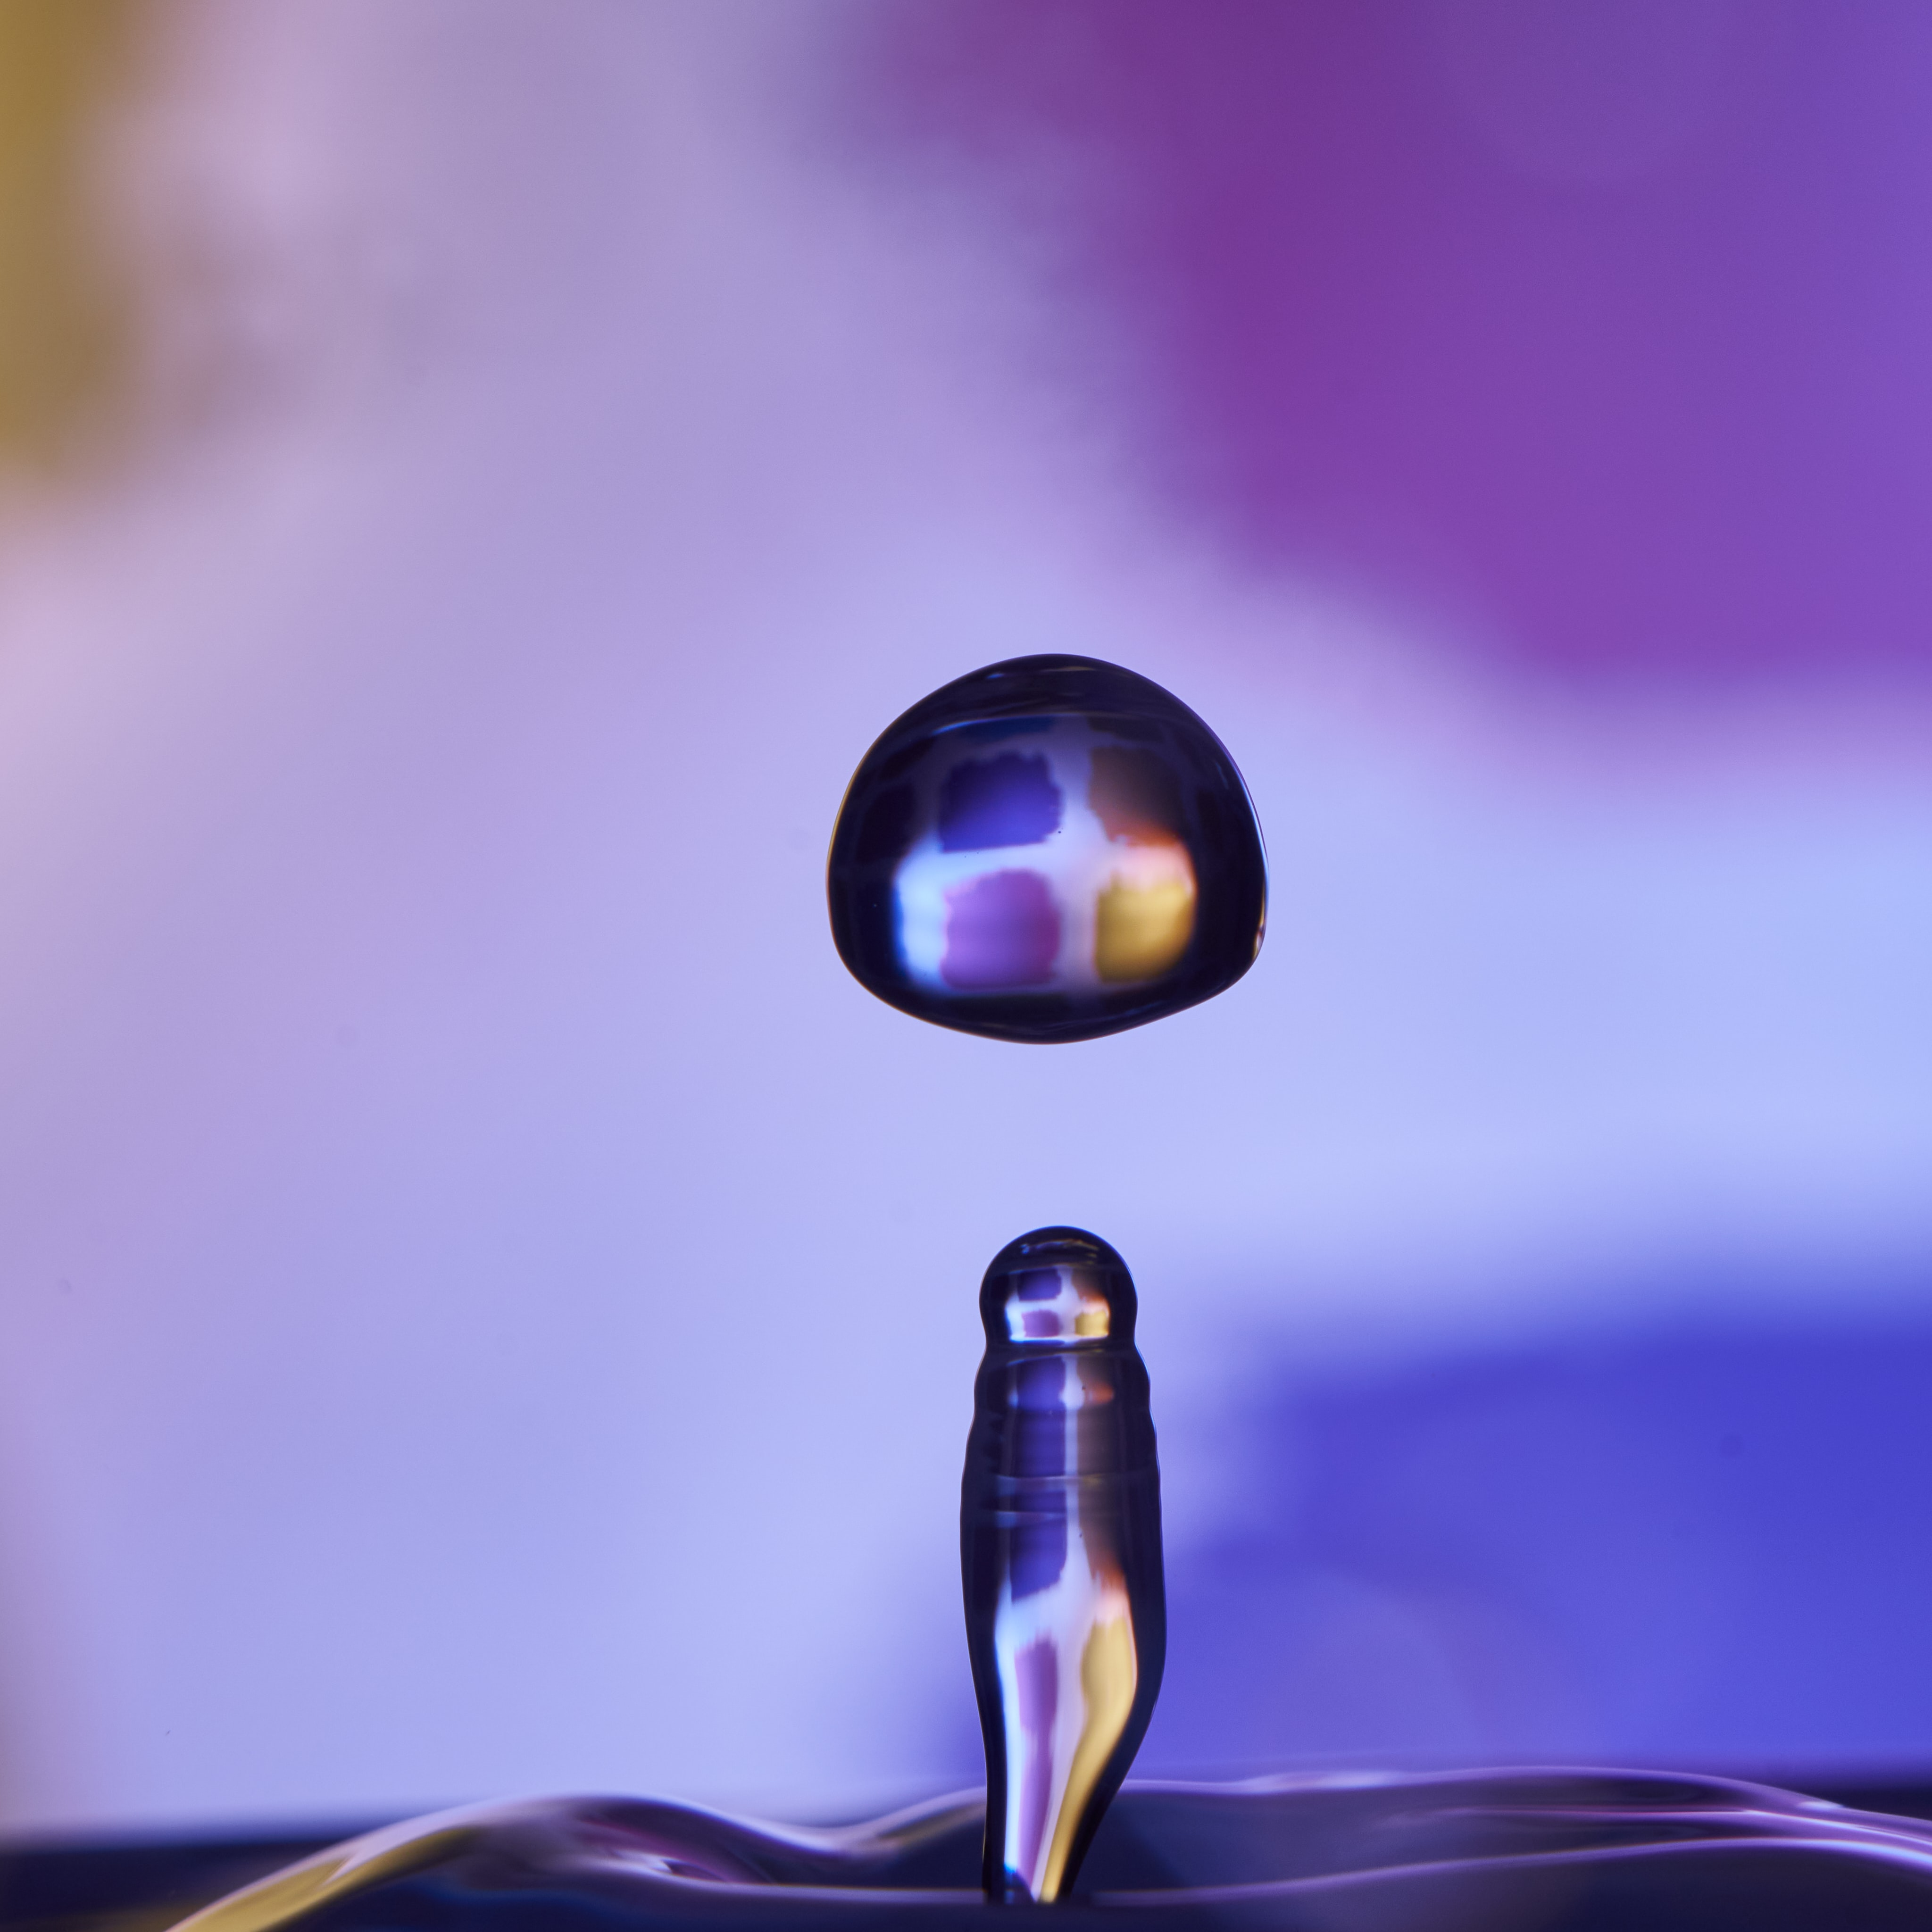
\includegraphics[height=4.8cm]{imgs/droplet_martin-brechtl-unsplash.png}
      \vskip.3cm
      Droplets are micron to millemetre sized liquid balls formed under surface tension.%
      \footnote<.->[frame]{Photo by Martin Brechtl on Unsplash.}
    \end{column}

    \pause
    \begin{column}{0.45\textwidth}
      \movie[showcontrols]{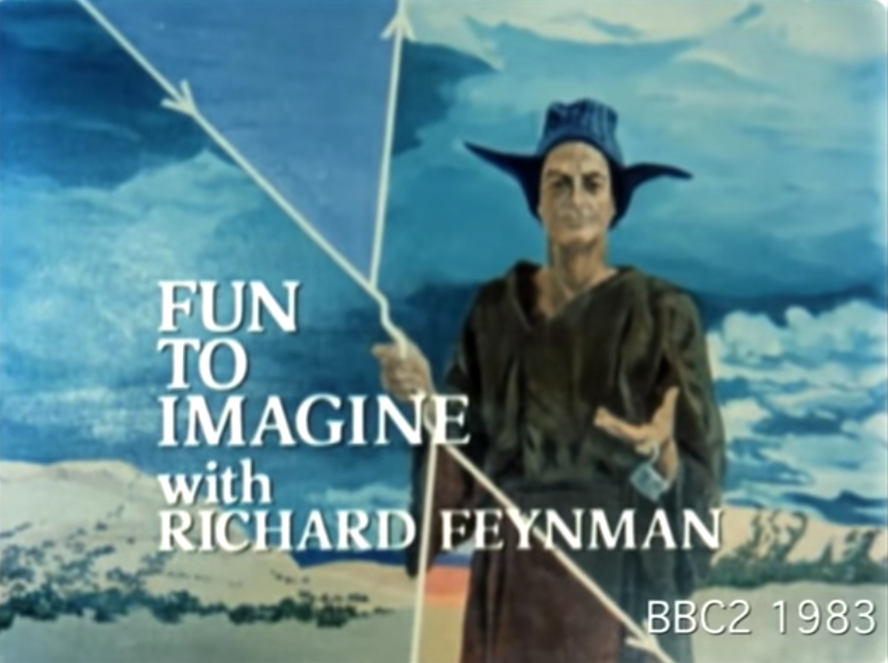
\includegraphics[height=4.8cm]{imgs/St_Feynman.png}}
            {videos/droplet-Feynman.mp4}
      \vskip.3cm
      BBC interview of Richard Feynman (1983).%
      \footnote<.->[frame]{Source: \texttt{https://youtu.be/P1ww1IXRfTA}.}
      
      \pause
      \vskip.3cm
      %\centering
      \textcolor{bb}{\bf Droplets are fun subjects!}
    \end{column}
  \end{columns}

  
\end{frame}

%% outline
\begin{frame}{Outline}
  \protect\hypertarget{outline}{}
  \tableofcontents
\end{frame}

%%
\hypertarget{part1}{%
  \section{Part I: Fabricating Photonic Crystals (PhC)}}

%% 
\hypertarget{background1}{%
  \subsection{Background, motivation and challenge}}

\begin{frame}
  \frametitle{Background, motivation and challenge}

  \emph{Photonic crystals} (PhC) are materials patterned with a periodicity in dielectric constant
  and show great potential for building sophisticated optical circuitry that can
  route, filter, store or suppress optical signals.
  \bigskip
  
  \begin{columns}[T]
    
    \begin{column}{0.6\textwidth}
      \begin{figure}
        \centering 
        \includegraphics[height=4.8cm]{imgs/photonic_crystal_fibre.png} 
        \caption{A scanning electron micrograph of a solid-core photonic crystal fibre and its far-field optical pattern.%
          \footnote<.->[frame]{P. Russell, Science: 358-362. (2003)}
          \textcopyright \enspace AAAS Science.}
      \end{figure}
    \end{column}
    \hskip0.5cm
    \pause
    \begin{column}{0.3\textwidth}
      \begin{figure}
        \centering 
        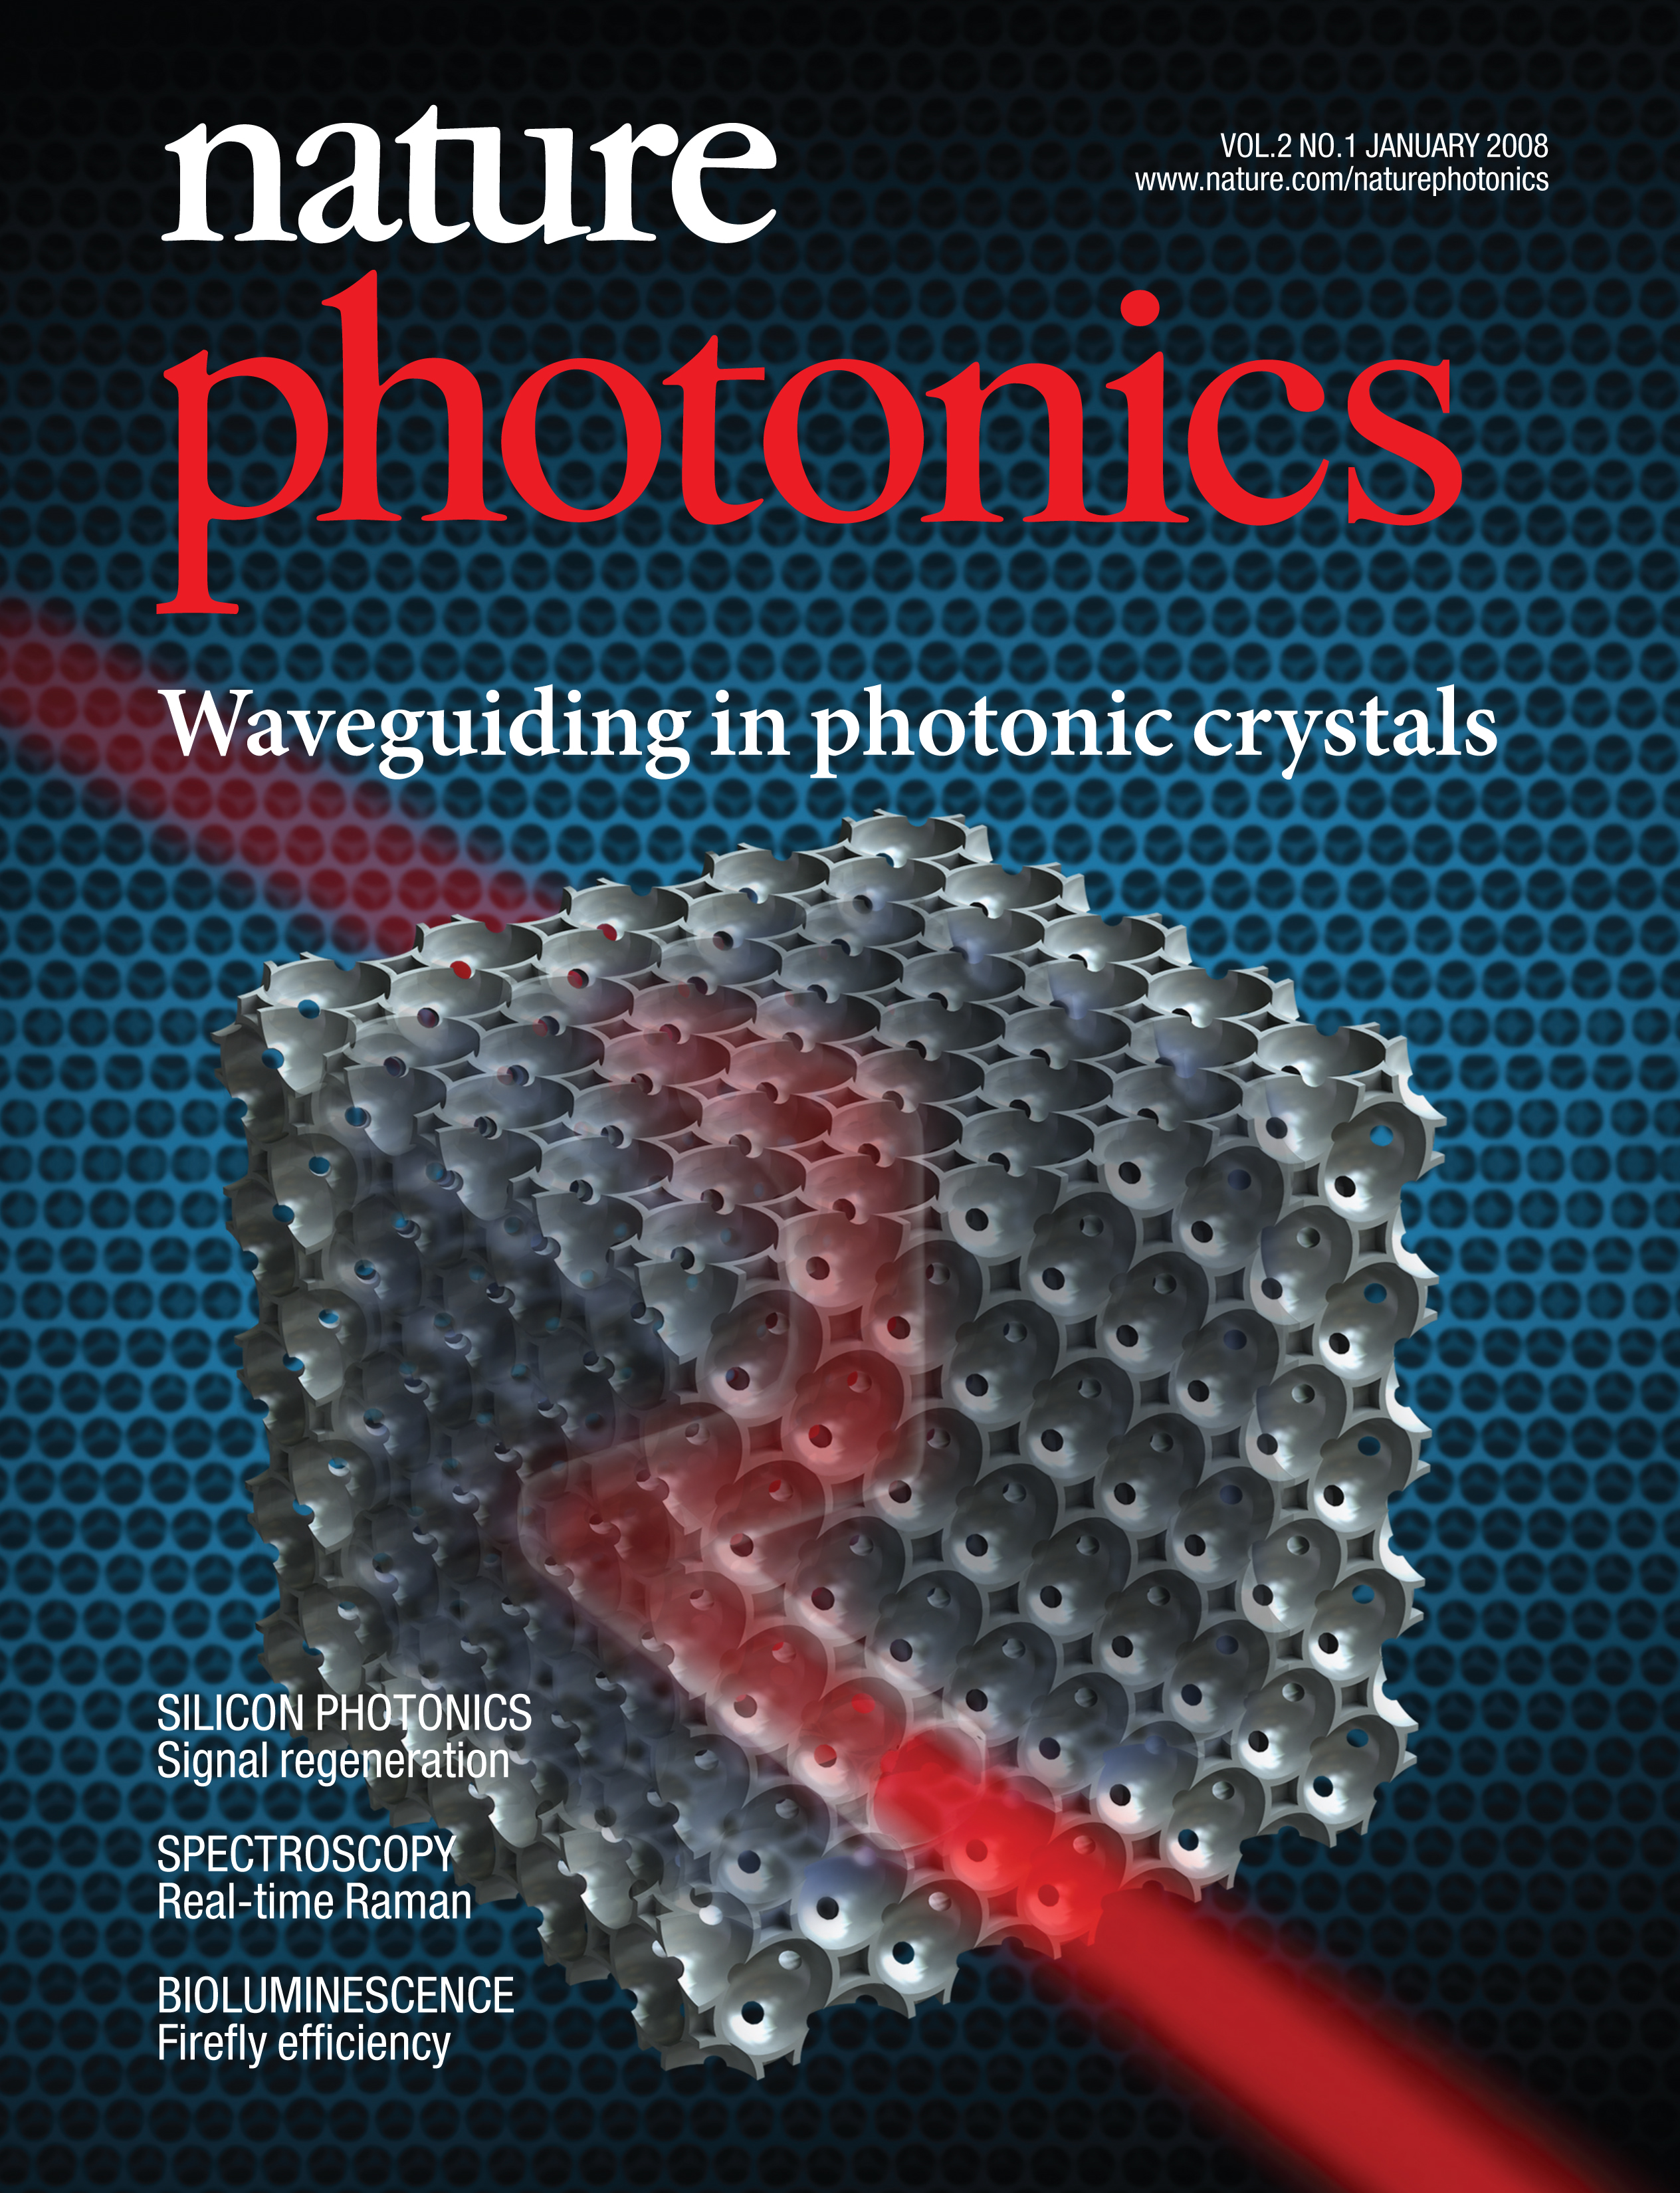
\includegraphics[height=4.8cm]{../imgs/photonics_cover.jpg} 
        \caption{An artistic rendering of a light beam passing through a 3D photonic crystal.
          \textcopyright \enspace Springer Nature (2008).}
      \end{figure}
    \end{column}
  \end{columns}
  
\end{frame}

\begin{frame}
  \frametitle{Background, motivation and challenge}

  Despite the theoretical promise, fabricating photonic crystals with 3D bandgaps is challenging in practice.
  \bigskip
  
  \pause
  \begin{columns}[T]
    \begin{column}{0.45\textwidth}
      \begin{figure}
        \centering
        \includegraphics[height=4.8cm]{imgs/diamond-111.png}
        \caption{A diamond cubic (view angle 111), ideal structure of PhC.}
      \end{figure}
    \end{column}

    \pause
    \begin{column}{0.45\textwidth}
      \begin{figure}
        \centering
        \includegraphics[height=4.8cm]{imgs/patchy_colloid.png}
        \caption{Self-assembly of micron-sized patchy particles mimicking the arrangements of bonds around atoms.
        \textcopyright \enspace Springer Nature (2012).}
      \end{figure}
    \end{column}

  \end{columns}
  \vskip0.1cm
  
  \pause
  \centering{
    \xb{\bf The obtained clusters may serve as basic building blocks for fabricating PhC.}
    \vskip0.08cm
    \pause
    \xr{\bf The challenge is to speed up the process.}}

\end{frame}

%%
\hypertarget{experiment}{%
  \subsection{Experiments, strategy and questions}}

\begin{frame}
  \frametitle{Experiments, strategy and questions}

  A few years ago, a series of experiments%
  \footnote{B. Shen \etal Exp. Fluids, 55, 1. (2014); B. Shen \etal Adv. Sci., 3: 1600012. (2016).}
  performed at ESPCI, Paris suggested an alternative approach...
  \bigskip
  \begin{columns}[T]
    
    \begin{column}{0.52\textwidth}
      \begin{figure}
        \centering 
        \movie[showcontrols]{\includegraphics[height=3cm]{imgs/espci-delta.png}}{videos/espci-3drops.mp4}
        \movie[showcontrols]{\includegraphics[width=6.5cm]{imgs/espci-tetra.jpg}}{videos/espci-4drops.mp4}
        \caption{Assembly of two to four droplets in a microfluidic chip.}
      \end{figure}
    \end{column}

    \pause
    \begin{column}{0.4\textwidth}
      \begin{figure}
        \centering 
        \includegraphics[height=4.5cm]{imgs/espci-cluster-morph.png}
        \caption{Observed cluster morphologies.
        Images courtesy of Dr.\ Bingqing Shen.}
      \end{figure}
    \end{column}

  \end{columns}
  
  \pause
  \xb{\bf Here, the droplet assembly is driven by the flow. Hence, it is much faster.} \vskip0.1cm
  \pause
  \xr{\bf The questions are why do they organize into such patterns and can we further optimize it?}
  
\end{frame}

%%
\hypertarget{dipolar}{%
  \subsection{A simple q2D dipolar model}}

\begin{frame}
  \frametitle{A simple q2D dipolar model}

  Noticing the strong geometric confinement of the microfluidic channel, physicists at ESPCI proposed the following \emph{dipolar model}.

  \begin{columns}[T]
    
    \begin{column}{0.45\textwidth}
      \centering
      \only<1-3,5,6>{\includegraphics[height=4cm]{imgs/espci-chip-cartoon.png}}
      \only<1-3>{\vskip.3cm \includegraphics[height=1.6cm]{imgs/espci-pancake.png}}
      \only<1-3>{\includegraphics[height=1.9cm]{imgs/espci-depletion.png}}
      \only<4>{\vskip.5cm 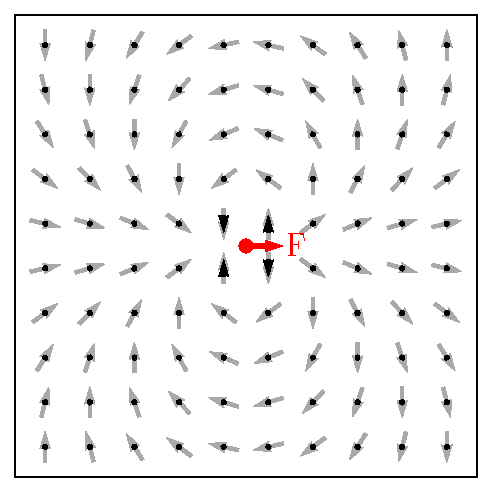
\includegraphics[height=6cm]{../imgs/dipolar.pdf}}
      \only<5,6>{\includegraphics[height=2.8cm]{imgs/espci-dipolar-cartoon.png} \\}
      \only<6>{\xr{\bf Is this picture really correct?}}
    \end{column}

    \pause

    \begin{column}{0.45\textwidth}
      
      \begin{bluecolorbox}[Obersvations \& hypotheses]
        \begin{itemize}
        \item Droplets are in quasi-two-dimensional (q2D) space.
        \item Depletion force attracts nearby drops.
        \item Hydrodynamic interactions (HI) lead to the rearrangement dynamics.
        \end{itemize}
      \end{bluecolorbox}

      \vskip.3cm
      \pause
      \begin{bluecolorbox}[Equations of motion (due to HI)]
        \begin{equation} \notag
          \begin{aligned}
            & {\bm u}^\infty(x,y,z) \approx -\frac{z(H-z)}{2\mu} \nabla p(x,y), \\
            & \delta{\bm u}_{ij} = {\bm B}_{ij} {\bm F}_j, \quad {\bm U}_i = {\bm u}^\infty_i + \sum_{j \ne i} \delta{\bm u}_{ij},
          \end{aligned}
        \end{equation}
        where
        \begin{equation} \notag
          \begin{aligned}
            {\bm B}({\bm x}) \approx -\frac{\alpha H}{\mu} \bigg( \frac{{\bm I}}{\abs{\bm x}^2} -
            \frac{ 2{\bm x}{\bm x} }{ \abs{{\bm x}}^4} \bigg).
          \end{aligned}
        \end{equation}
      \end{bluecolorbox}
    \end{column}

  \end{columns}
    
\end{frame}

%%
\hypertarget{simulation1}{%
  \subsection{3D numerical simulations}}

\begin{frame}
  \frametitle{3D numerical simulations}

  To verify the model and subsequently optimize the chip design, we set up direct numerical simulations (DNS) of droplets in microchannels.
  \vskip0.3cm

  \pause
  \begin{columns}[T]

    \begin{column}{0.55\textwidth}
      \begin{bluecolorbox}[Mathematical formulation]
        The incompressible Navier-Stokes (NS) equations read,
        \begin{subequations} \label{eq:Navier-Sotkes}
          \begin{equation}
            \nabla \cdot {\bm u} = 0,
            \label{eq:div-free}
          \end{equation}
          \begin{equation}
            \rho \bigg(\frac{\partial {\bm u}}{\partial t} + {\bm u} \cdot \nabla {\bm u} \bigg) = \nabla \cdot {\bm \sigma} + {\bm f},
            \label{eq:NS}
          \end{equation}
        \end{subequations}
        where $\bm \sigma$ is the viscous stress tensor, given as
        \begin{equation}
          \begin{aligned}
            {\bm \sigma} = -p {\bm I}+ \mu \bigg( \nabla {\bm u} + (\nabla {\bm u})^T \bigg),
          \end{aligned}
        \end{equation}
        and is subject to the following boundary condition across the interface
        \begin{equation} \label{eq:stress-bc}
          ({\bm \sigma}_+ - {\bm \sigma}_- ) \cdot {\bm n} = \gamma \kappa {\bm n} - \nabla \gamma.
        \end{equation}
      \end{bluecolorbox}
    \end{column}

    \pause
    \begin{column}{0.4\textwidth}
      \centering
      \begin{bluecolorbox}[Non-dimensional numbers]
        \begin{equation} \notag
          \begin{aligned}
            \textrm{Re} = \frac{\rho UL}{\mu}, \quad
            \textrm{Ca} = \frac{\mu U}{\gamma}, \quad
            \textrm{Fr} = \frac{U^2}{FL}.  
          \end{aligned}
        \end{equation}
      \end{bluecolorbox}
      \vskip0.2cm

      \pause
      \begin{flushleft}
        In the experiments, %Re $\sim 10^{-2}$, Ca $\sim 10^{-5}$, Fr $\sim 10^{-5}$,
        \begin{equation} \notag
          \begin{aligned}
            \textrm{Re} \sim 10^{-2}, \quad
            \textrm{Ca} \sim 10^{-5}, \quad
            \textrm{Fr} \sim 10^{-5}.  
          \end{aligned}
        \end{equation}
        It means that inertial effects are negligible,
        the droplets will remain mostly spherical,
        and gravity matters.
        \vskip0.4cm

        \pause
        In developing the numerical solver, no such assumptions are made.
      \end{flushleft}
    \end{column}
    
  \end{columns}
  
\end{frame}

%%
\hypertarget{icls}{%
  \subsubsection{ICLS/GFM}}
%%1
\begin{frame}[t]
  \frametitle{Interface-resolved one-fluid methods}

  \begin{columns}[T]

    \begin{column}{0.45\textwidth}
      \vskip0.2cm
      \only<1-4>{
      There are numerous methods for direct simulation of droplets in fluids, such as
      \medskip
      \begin{itemize}
      \item the front-tracking methods
      \item the volume-of-fluid methods    
      \item the level set (LS) methods
      \item the phase field methods
      \item the lattice-Boltzmann methods
      \item the boundary integral methods
      \item ...
      \end{itemize}
      } % end only
      \medskip
      \only<2-4>{We use {\bf LS} for its simplicity and mathematical convenience.}

      \medskip
      \only<4>{However, there is an \xr{issue}...}
      \only<5->{\movie[showcontrols,poster,width=6cm,height=6.5cm]{}{videos/serpentine.mp4} \vskip0.2cm}
      \only<6->{\hskip1.2cm \xr{\bf LS is not mass-conserving.}}
      
    \end{column}

    
    \begin{column}{0.5\textwidth}
      \only<3->{
      \begin{bluecolorbox}[Classical LS formulation]

        The level set function, $\phi$, is classically defined as the signed distance to the interface $\Gamma$,
        \begin{equation} 
          \phi({\bm x},t) = sgn({\bm x}) |{\bm x}-{\bm x}_\Gamma|.
        \end{equation}
        For example, a sphere of radius r centered at origin can be represented as
        \begin{equation} \notag
          \Gamma = \{ {\bm x} ~ \rvert ~ \phi({\bm x},t) = 0 \},
        \end{equation}
        where
        \begin{equation} \notag
          \phi({\bm x},t) = |{\bm x}|^2 -r.
        \end{equation}
        The normal and the curvature of the interface can be readily calculated as
        \begin{equation}
          {\bm n} = \nabla \phi / \abs{ \nabla \phi }, \quad \kappa = \nabla \cdot {\bm n}.
        \end{equation}
        The interface motion is governed by
        \begin{equation} \label{eq:ls-avd}
          \frac{\partial \phi}{\partial t} + \bm{u} \cdot \nabla \phi = 0.
        \end{equation}
        
      \end{bluecolorbox}
      } %end only
    \end{column}
    
  \end{columns}

\end{frame}
%%2
\begin{frame}[t]
  \frametitle{Interface-correction level set/ghost fluid method (ICLS/GFM)}
  
  \begin{columns}[T]

    \begin{column}{0.45\textwidth}
      \vskip0.2cm
      \only<1->{
      To remedy the problem, we developed a simple mass-correction scheme.%
      \footnote<.->[frame]{Z. Ge \etal J. Comput. Phys. 353: 435-459. (2018)}
      } % end only
      \vskip0.2cm
      \only<2->{
      The key idea is to construct a correction-velocity, ${\bm u}_c$,
      such that the total volume is controlled by doing an additional advection.
      \vskip0.2cm} % end only
      \only<4>{\centering{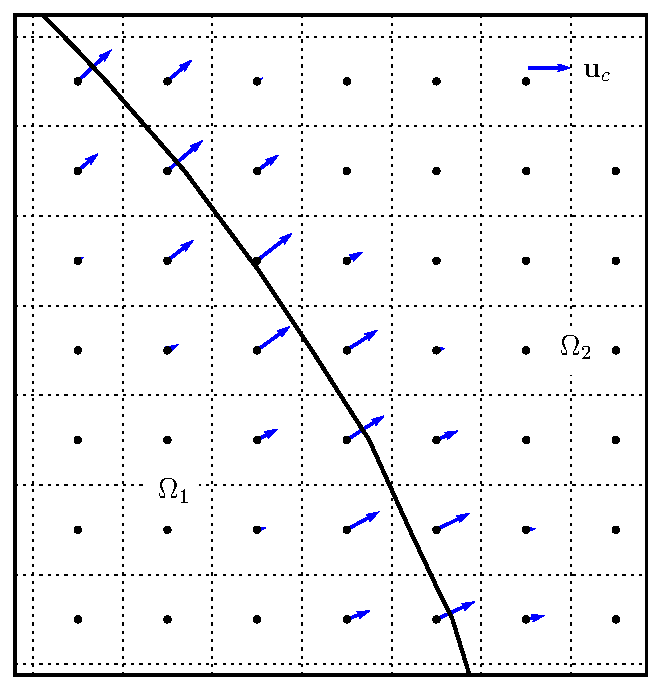
\includegraphics[width=0.75\textwidth]{../paper1/Figures/mc.pdf}}} % end only
    \end{column}

    
    \begin{column}{0.5\textwidth}
      \only<3->{
      \begin{bluecolorbox}[ICLS formulation]

        The level set is defined and evolved in the same way as in the classical formulation,
        except that we also periodically examine the fluid mass loss.
        This allows us to define ${\bm u}_c$ as
        \begin{equation} \notag
          \int_\Gamma {\bm n} \cdot {\bm u}_c \,d\Gamma = \frac{\delta V}{\delta t},
        \end{equation}
        where $-\delta V/\delta t$ corresponds to the mass loss over an arbitrary period of time.
        If ${\bm u}_c$ is known, then solving
        \begin{equation}
          \frac{\partial \phi}{\partial t} + {\bm u}_c \cdot \nabla \phi = 0,
        \end{equation}
        will remove the mass loss accumulated over $\delta t$.

        It can be shown that
        \begin{equation}
          {\bm u}_c(\phi) = \frac{\delta V}{\delta t} \frac{\kappa(\phi)}{A_f} \delta_\epsilon (\phi),
        \end{equation}
        where $A_f = \int_\Gamma f_s \delta_\epsilon (\phi)|\nabla \phi| \,d\Gamma$.
        
      \end{bluecolorbox}
      } %end only
    \end{column}
    
  \end{columns}

\end{frame}
%%3
\begin{frame}[noframenumbering]
  \frametitle{Interface-correction level set/ghost fluid method (ICLS/GFM)}

  \centering
  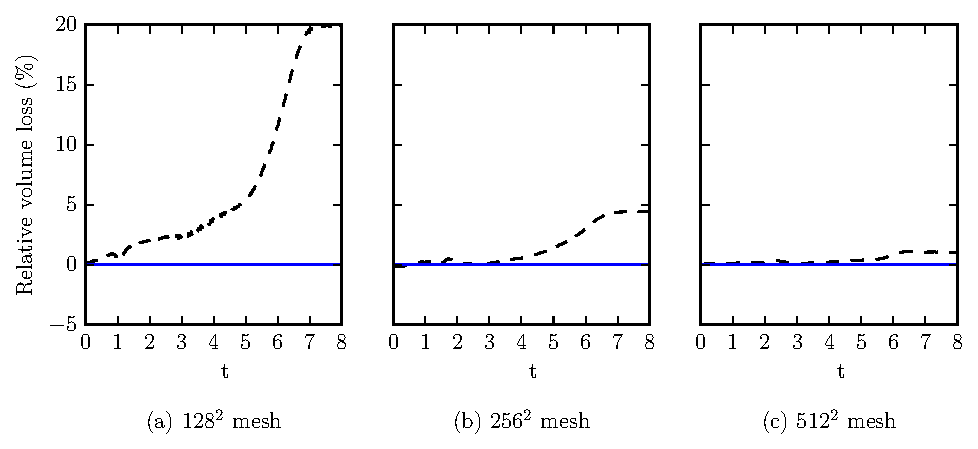
\includegraphics[width=0.8\textwidth]{../paper1/Figures/serp_loss.pdf}
  \vskip0.3cm
  \pause
  \xb{\bf A global mass conservation is now achieved.}

\end{frame}
%%4
\begin{frame}[noframenumbering]
  \frametitle{Interface-correction level set/ghost fluid method (ICLS/GFM)}

  \begin{columns}[T]
    
    \begin{column}{\textwidth}
      The flow solver also requires accurate computation of surface tension... \vskip0.2cm
      and a hydrodynamic model to impose the depletion force ... \vskip0.2cm
      \pause
      These details are given in: \vskip0.5cm
      \centering
      \begin{tcolorbox}[beamer,
          width=0.7\textwidth,
          arc=0pt,
          boxsep=1pt,
          left=0pt,right=0pt,top=0pt,bottom=0pt,
        ]
        \includegraphics[width=\linewidth]{imgs/JCP-cover.png}
      \end{tcolorbox}
    \end{column}
  \end{columns}

\end{frame}  
%%5
\begin{frame}[noframenumbering]
  \frametitle{Interface-correction level set/ghost fluid method (ICLS/GFM)}
  
  \begin{columns}
    
    \begin{column}{0.7\textwidth}
      \vskip0.3cm
      \only<1->{
      \begin{algorithm}[H] \notag
        \ccc{\footnotesize //time marching} \\
        \For{$n=1,2,\dots,N$}{
          
          \ccc{\footnotesize //level set advection} \\
          $\phi^1 = \phi^{(n)} + \Delta t \cdot {AD}(\phi^{(n)})$ \\
          $\phi^2 = \frac{3}{4} \phi^{(n)} + \frac{1}{4} \phi^1 + \frac{1}{4} \Delta t \cdot {AD}(\phi^1)$ \\
          $\phi^{(n+1)} = \frac{1}{3} \phi^{(n)} + \frac{2}{3} \phi^2 + \frac{2}{3} \Delta t \cdot {AD}(\phi^2)$ \\
              {\small Calculate $\rho^{(n+1)}$, $\mu^{(n+1)}$, $\bm{n}$, and $\kappa$ using $\phi^{(n+1)}$ } \\

              \ccc{\footnotesize //correct and reinitialize the level set every $N_i$ steps} \\
              \If{$n \mod N_i =0$}{
                {\small Mass-correction: advect with ${AD}(\phi) = (\delta V/\delta t) (\kappa \delta(\phi)/A_f)$} \\
                {\small Reinitialization: advect with ${AD}(\phi) = S(\phi)(\abs{\nabla \phi} -1)$} \\
              }
              \ccc{\footnotesize //flow solver (AB2)} \\
              ${\bf RU}^{(n)} = -{\bm u}^{(n)} \cdot \nabla {\bm u}^{(n)} +\frac{1}{Re}\big(\frac{1}{\rho^{(n+1)}} \nabla \cdot \big[\mu^{(n+1)}(\nabla {\bm u}^{(n)}+(\nabla {\bm u}^{(n)})^T)\big]\big)$ \\
              ${\bm u}^* ={\bm u}^{(n)} +\Delta t \big(\frac{3}{2} {\bf RU}^{(n)}-\frac{1}{2} {\bf RU}^{(n-1)} \big)$ \\
              $\nabla ^2 p^{(n+1)} = \nabla ^2_g [p]_\Gamma + \nabla \cdot \big[ \big(1-\frac{\rho_0}{\rho^{(n+1)}}) \nabla_g \hat{p} \big] + \frac{\rho_0}{\Delta t} \nabla \cdot {\bm u}^*$ \ccc{\footnotesize //FastP*-GFM} \\
              ${\bm u}^{(n+1)} = {\bm u}^* -\Delta t \big[\frac{1}{\rho_0} \nabla_g p^{(n+1)} + \big(\frac{1}{\rho^{(n+1)}} - \frac{1}{\rho_0}\big) \nabla_g \hat{p} \big]$ \ccc{\footnotesize //correction} \\
              ${\bf RU}^{(n-1)}={\bf RU}^{(n)}$ \\
        }
        \caption{A pseudo-code of ICLS/GFM.}
      \end{algorithm}
      }%end only
    \end{column}
    
    \begin{column}{0.2\textwidth}
      \only<2->{
        \vskip5.5cm
        \centering
        \includegraphics[width=1.2cm]{imgs/github.png}
        \vskip0.1cm
        Available at \texttt{ICLS-release}
      } %end only
    \end{column}
  \end{columns}

\end{frame}
%%5
\begin{frame}[noframenumbering]
  \frametitle{Interface-correction level set/ghost fluid method (ICLS/GFM)}

  \begin{columns}
    
    \begin{column}{0.9\textwidth}
      
      \begin{bluecolorbox}[Summary of numerics]
        \medskip
        \begin{itemize}
        \item The LS part is solved by standard techniques for hyperbolic partial differential equations. \medskip
        \item The NS part is solved by a standard projection method. \medskip
        \item The equations are solved on a staggered Cartesian grid using the finite volume method. \medskip
        \item The temporal integration is the 2nd-order Adam-Bashforth scheme. \medskip
        \item The pressure Poisson equation is solved using a fast Fourier transform based solver. \medskip
        \item The pressure jump across an liquid interface is imposed by the ghost fluid method (GFM). \medskip
        \item The depletion force between droplets is also computed under the GFM framework. \medskip
        \end{itemize}
      \end{bluecolorbox}
       
    \end{column}
    
  \end{columns}

  \vskip0.5cm
  \pause
  \centering
  \xb{\bf Now, we are ready to simulate the droplets.}
  
\end{frame}

%%%
%\hypertarget{ibm}{%
%  \subsubsection{NS/IBM}}


%%
\hypertarget{assembly}{%
  \subsection{Flow-assisted assembly}}

\begin{frame}[t]
  \frametitle{Flow-assisted assembly}

  \begin{columns}[T]
    
    \begin{column}{0.5\textwidth}      
      \only<1->{In our microfluidic device, the droplet dynamics are governed by:
      \vskip0.3cm
      \begin{itemize}
      \item near-field depletion force
      \item shear
      \item confinement
      \item boundary condition
      \end{itemize}
      \vskip0.3cm} %end only
      \only<2>{We examine these effects one-by-one as in the paper below.}
    \end{column}

    \begin{column}{0.45\textwidth}
      \only<1->{
      \centering
      \includegraphics[height=4cm]{imgs/espci-chip-cartoon.png}} %end only
    \end{column}
    
  \end{columns}
  
  \only<2>{
    \begin{textblock}{160}(12,54)
      \begin{tcolorbox}[beamer,
          width=.6\textwidth,
          arc=0pt,
          boxsep=1pt,
          left=0pt,right=0pt,top=0pt,bottom=0pt,
        ]
        \includegraphics[width=\linewidth]{imgs/soft-mat.png}
      \end{tcolorbox}
    \end{textblock}
  } %end only
    
\end{frame}

%%1
\begin{frame}[t]
  \frametitle{Flow-assisted assembly: Approaching droplets in quiescent flows}

  \begin{columns}[T]
    \begin{column}{0.55\textwidth}
      Dimensional analysis suggests the following scaling.  \vskip0.2cm
      \begin{itemize}
      \item The strength of the attraction $\propto \Pi=p_{os}/p$.
      \item The approaching time $\propto T_\pi = r_s/(R\Pi)$.
        \only<3->{\item The physical time scale, $\tau_\pi = r_s \mu /(R p_{os})$, is $\sim 1$ ns.%
          \footnote<3->[frame]{Typical experimental values:
            $r_s = 1$ nm, ${\mu} = 10^{-3}$ kg/m-s, ${R} = 10$ $\mu$m, and ${p}_{os} = 100$ Pa.}
          }
        \only<4->{\\ Therefore, the approaching can be considered instantaneous.}
      \end{itemize}
    \end{column}

    \begin{column}{0.4\textwidth}
      \begin{figure}
        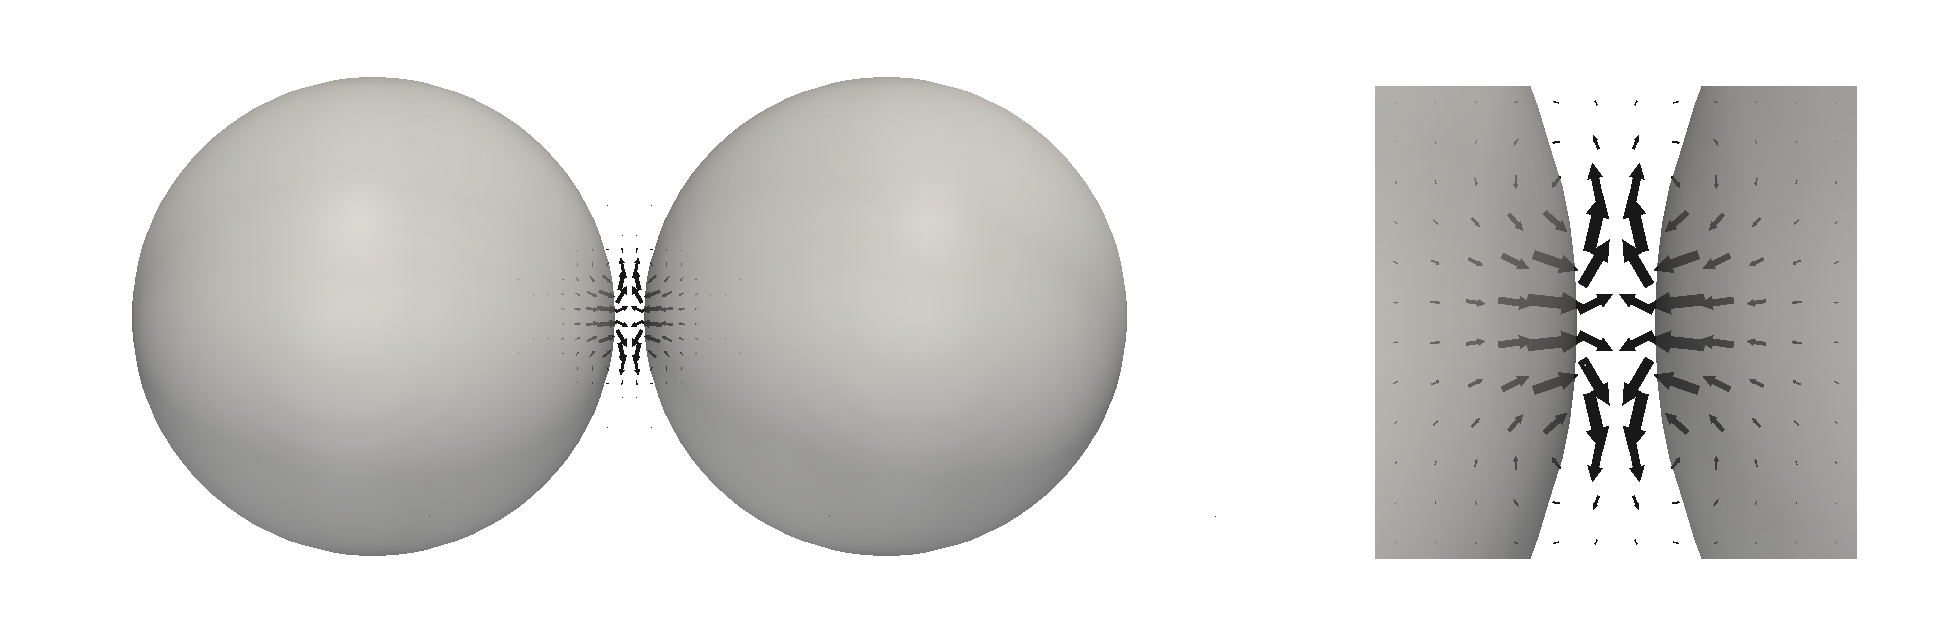
\includegraphics[width=\columnwidth]{../paper2/figs/depletion_flow.png}
      \end{figure}

    \end{column}
    
  \end{columns}

  \vskip0.4cm
  \only<2-3>{
    \begin{figure}
      \centering
      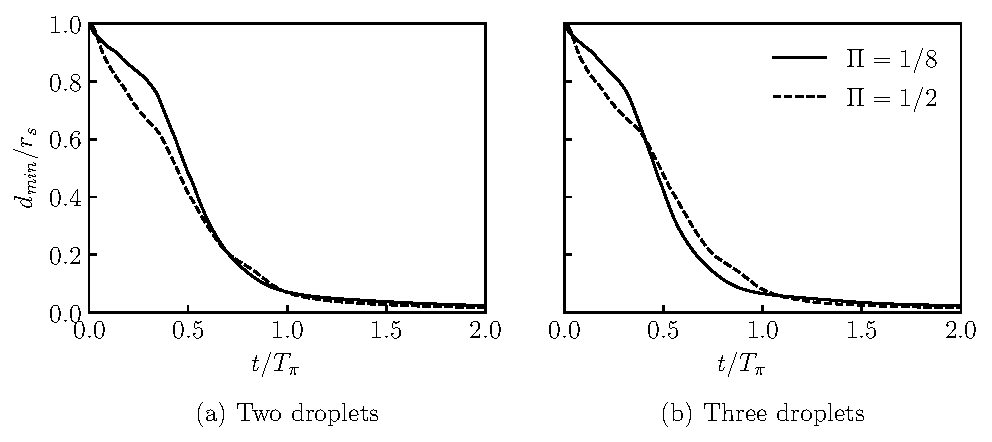
\includegraphics[width=0.75\textwidth]{../paper2/figs/min_dist4.pdf}
      \begin{picture}(0,0)
        \put(-210,48){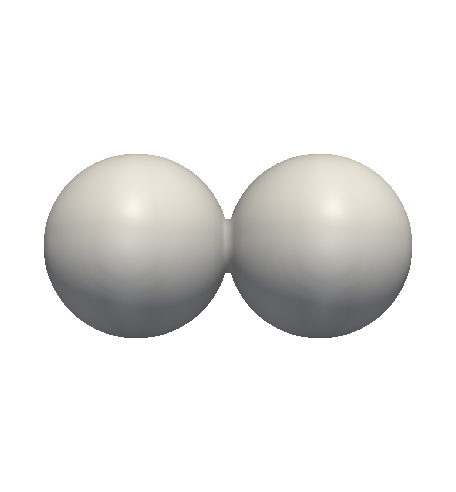
\includegraphics[height=1.4cm]{../paper2/figs/2dp.png}}
        \put(-55, 48){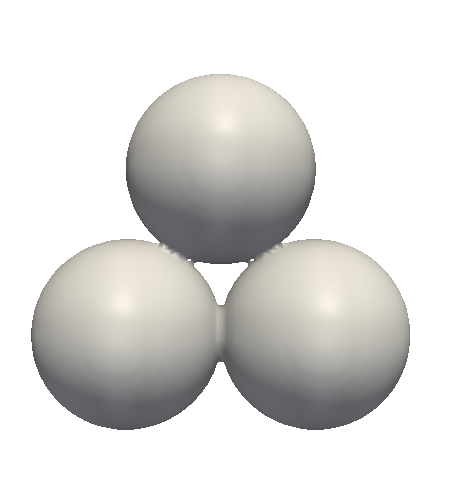
\includegraphics[height=1.4cm]{../paper2/figs/3dp.png}}
      \end{picture}
    \end{figure}
  } %end only

  \only<5>{
    \begin{figure}
      \centering
      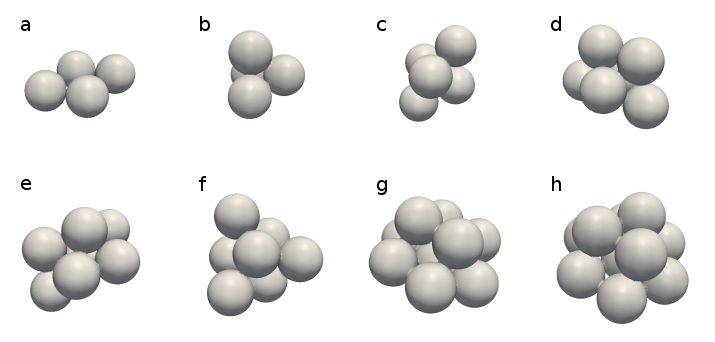
\includegraphics[width=0.6\textwidth]{../paper2/figs/packings.png}
    \end{figure}
  } %end only

  \only<6>{ \vskip0.6cm
    \begin{columns}    
      \begin{column}{0.7\textwidth}
        \begin{bluecolorbox}[Characteristics of depletion force]
          In summary, the depletion attraction
          \medskip
          \begin{itemize}
          \item is local (activated at nearly touching);
          \item acts in the radial direction; 
          \item has a fast relaxation time. 
          \end{itemize}
          \medskip
          Consequently, the effect of depletion force on cluster morphology is to preserve the initial positions in the absence of noise. 
        \end{bluecolorbox}
      \end{column}
    \end{columns}
  }
    
\end{frame}

%%2
\begin{frame}[t]
  \frametitle{Flow-assisted assembly: Sticky droplets in shear-driven channel flows}

  \vskip0.4cm
  \only<1->{
    \begin{columns}[c]
      \begin{column}{.3\textwidth}
        A pair of droplets in unbounded simple shear flow has two types of trajectories%
        \footnote<.->[frame]{Batchelor \& Green, J. Fluid. Mech. 56, (2), 375-400. (1972).}: \medskip
        \begin{itemize}
        \item open trajectory;
        \item closed trajectory.
        \end{itemize}
      \end{column}
      
      \begin{column}{.6\textwidth}
        \centering 
        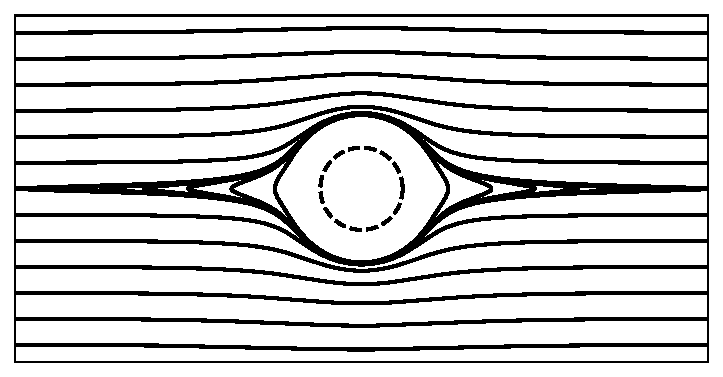
\includegraphics[width=.8\columnwidth]{../imgs/BG-traj4.pdf}
        
      \end{column}
    \end{columns}
  } %end only

  \vskip0.4cm  
  \only<2->{These two classes of trajectory is only determined by the relative position for equal spheres.\\} 
  \only<3->{Adding a depletion force shall not alter the phase portrait, since the force is local.}
  
  \vskip0.4cm  
  \only<4->{\xb{However, adding both depletion and confinement will change the droplet dynamics.} \\
    (Actually, adding confinement alone already changes the picture qualitatively.%
    \footnote<4->[frame]{M. Zurita-Gotor \etal J. Fluid. Mech. 592, 447-469. (2007). I. Fouxon \etal ArXiv:1908.11208.})}

  %\vskip0.4cm
  %\only<5->{\xr{\bf What is the nature of droplet interactions under depletion force and shear in strongly confined geometries?}}  
    
\end{frame}

%%2.0
\begin{frame}[t,noframenumbering]
  \frametitle{Flow-assisted assembly: Sticky droplets in shear-driven channel flows}

  We simulate a pair of touching droplets in a shear-driven channel of height $L_z=1.5D$. \vskip0.2cm
  Without the depletion attraction, droplets separate and swap their positions (i.e.\ symmetrical). \vskip0.2cm
  
  \begin{figure}
    \centering
    \movie[]{\includegraphics[width=.5\columnwidth]{imgs/shear.png}}
          {videos/shear-swap-no-depl.ogv}
  \end{figure}

\end{frame}

%%2
\begin{frame}[t,noframenumbering]
  \frametitle{Flow-assisted assembly: Sticky droplets in shear-driven channel flows}

  We simulate a pair of touching droplets in a shear-driven channel of height $L_z=1.5D$. \vskip0.2cm
  Without the depletion attraction, droplets separate and swap their positions (i.e.\ symmetrical). \vskip0.2cm
  With the depletion attraction, only one configuration is dynamically stable (i.e.\ the symmetry is lost). \vskip0.5cm

  \only<1-2>{
  \begin{figure}
    \centering
    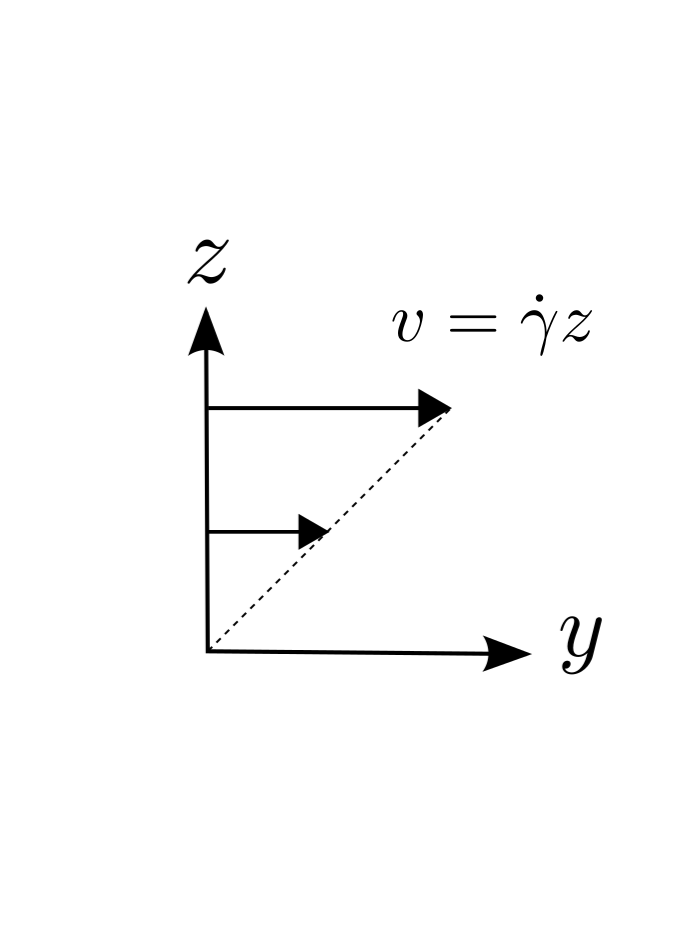
\includegraphics[width=.15\columnwidth]{../paper2/figs/shear1.png}
    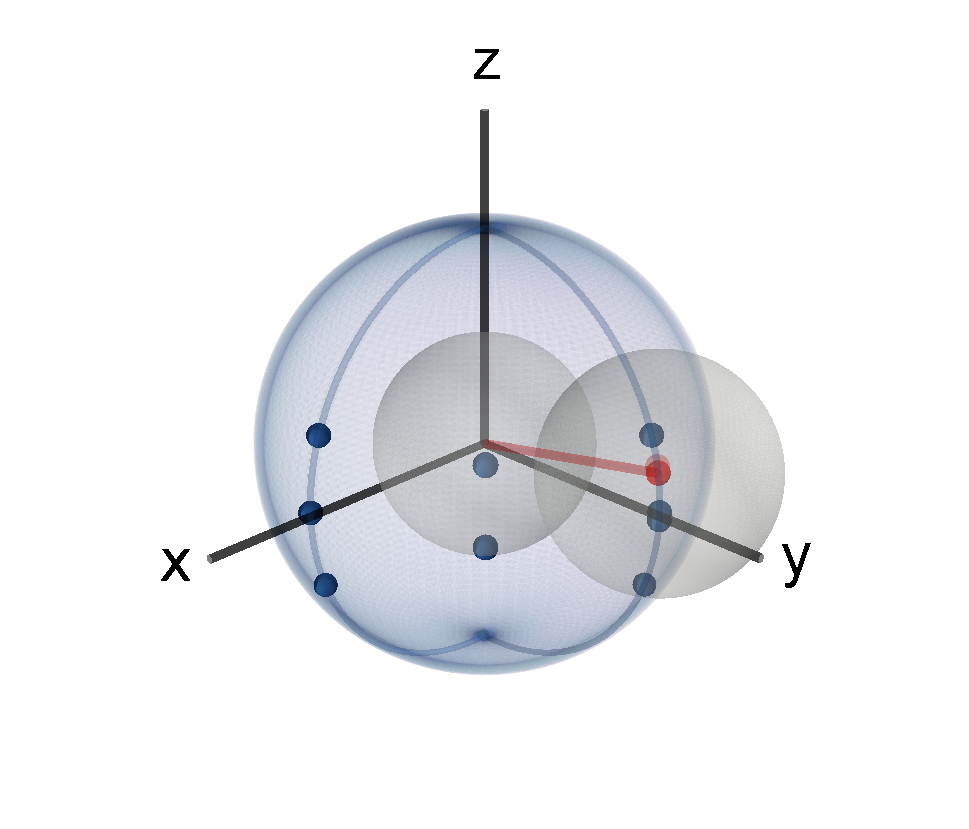
\includegraphics[width=.32\columnwidth]{../paper2/figs/shell1.png} %\vskip0.1cm
    \only<1>{
      \movie[]{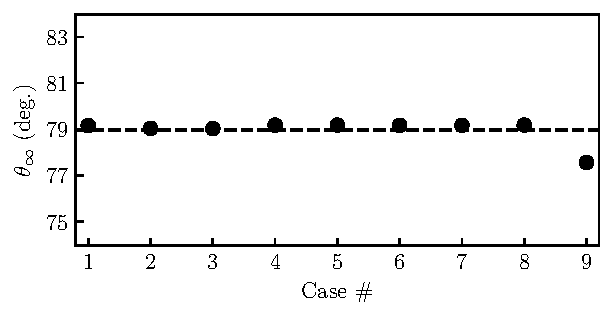
\includegraphics[width=.4\columnwidth]{../paper2/figs/angle_final2.pdf}}
            {videos/shear-align-case8.ogv} } %end only
    \only<2>{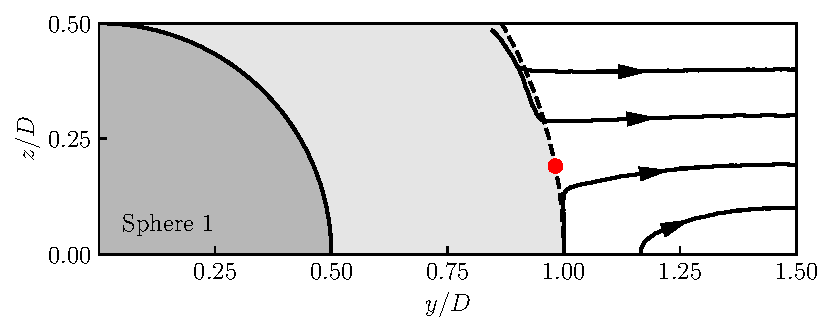
\includegraphics[width=.415\columnwidth]{../paper2/figs/traj.pdf}}
    \caption{All initial positions (\xb{blue dots}) stabalize at a polar angle $\theta_\infty=$ 79 deg (\xr{red dot}).}
  \end{figure} }%end only

  \only<3>{
    \vskip1cm
    \begin{columns}
      \begin{column}{0.6\textwidth}
        
        \begin{bluecolorbox}[Effects of depletion force $+$ shear $+$ confinement]
          \medskip
          \begin{itemize}
          \item It is a symmetry-breaking mechanism even at $N=2$. \medskip
          \item It leads to alignment in the flow direction. \medskip
          \item When $N>2$, we expect a chain of droplets. \medskip
          \end{itemize}
        \end{bluecolorbox}
        
      \end{column}
    \end{columns}
  } %end only

\end{frame}

%%
\begin{frame}[t]
  \frametitle{Flow-assisted assembly: Droplet clusters in pressure-driven channel flows}

  Finally, we turn to pressure-driven channel flows. \vskip0.2cm
  \only<2-5>{In the region far away from the inlet...} %\vskip0.2cm
  \only<6->{In the region close to the inlet...} \vskip0.2cm
  
  \begin{columns}

    \begin{column}{0.4\textwidth}
      \only<1-7>{
      \begin{textblock}{60}(10,35)
        \includegraphics{imgs/espci-chip-cartoon.png}
      \end{textblock}
      } %end only
      \only<8>{
        \begin{bluecolorbox}[Effects of all combined]
          \medskip
          \begin{itemize}
          \item Uniform flow favors chain-like structures. \medskip
          \item Non-uniform flow promotes compact structures. \medskip
          \item Overall, these are 3D effects. \medskip
          \end{itemize}
        \end{bluecolorbox}
      } % end only
    \end{column}

    \begin{column}{0.5\textwidth}
      \begin{figure}
      %\centering
      \only<2>{
        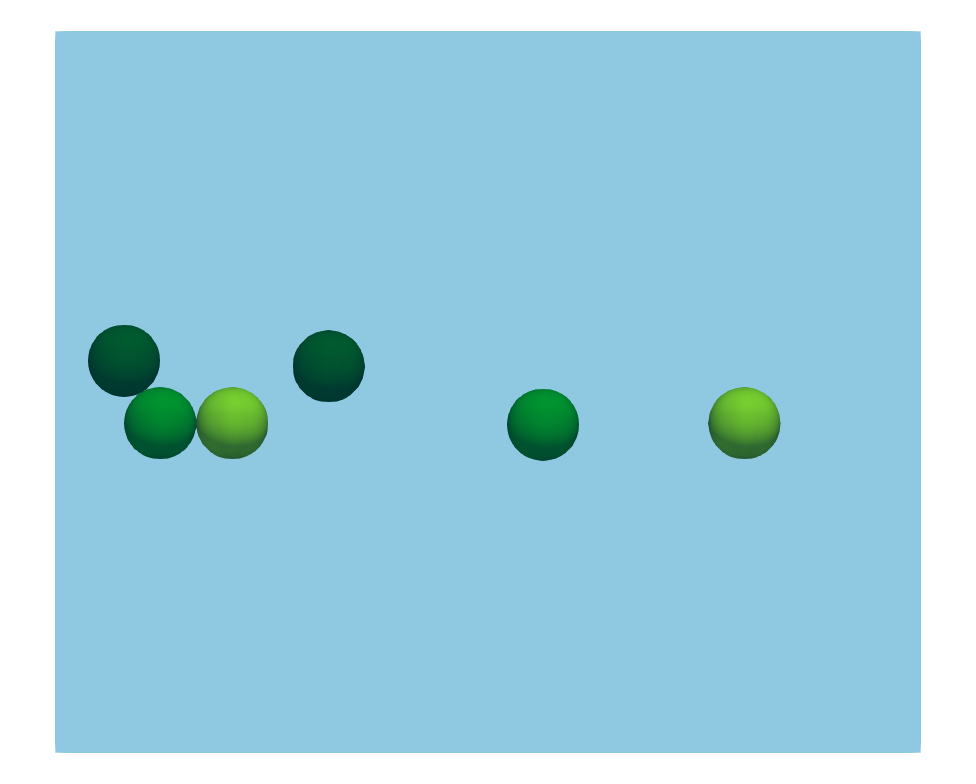
\includegraphics[width=.7\columnwidth]{../paper2/figs/3-scatter-top.png}
        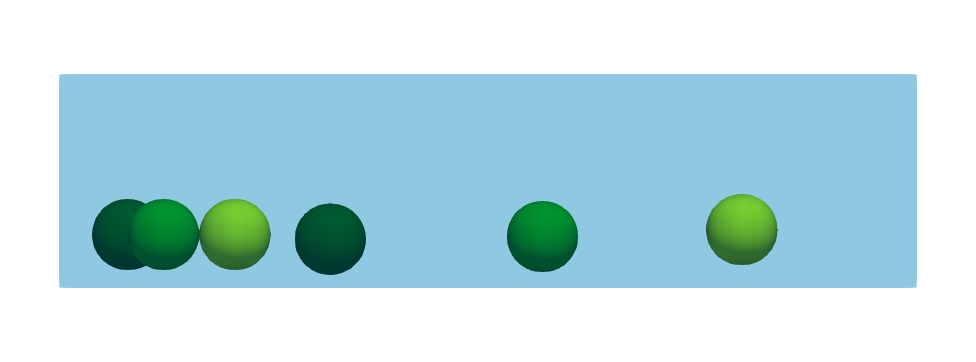
\includegraphics[width=.7\columnwidth]{../paper2/figs/3-scatter-side.png}
        \vskip0.3cm
        Without depletion force: scattering drops.
      } % end only
      \only<3>{
        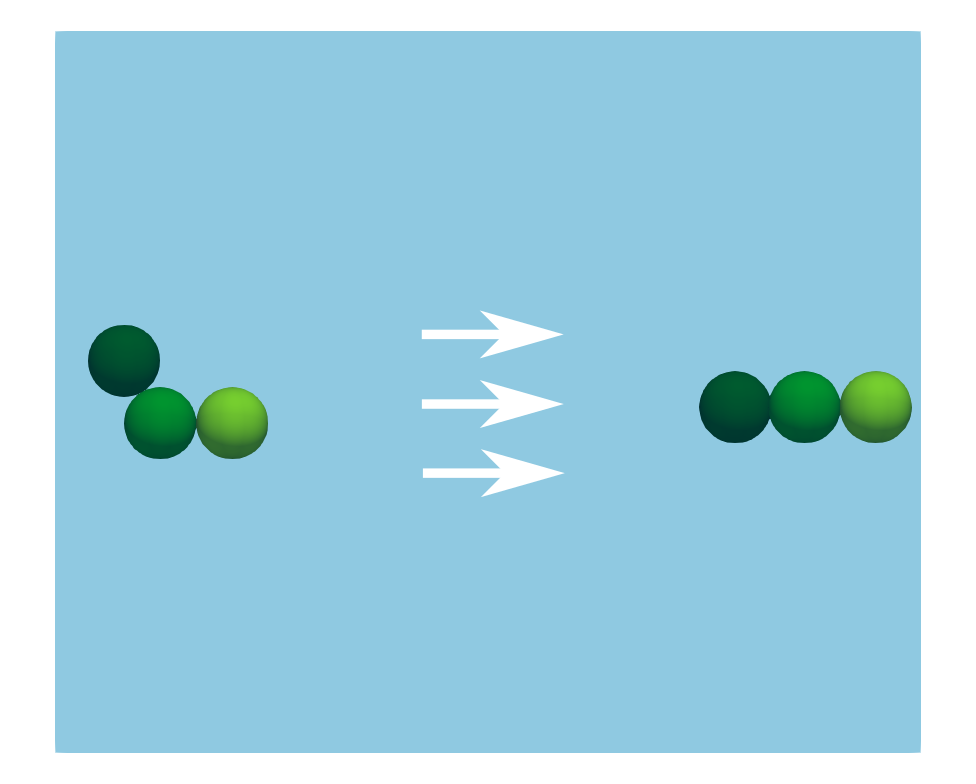
\includegraphics[width=.7\columnwidth]{../paper2/figs/3-line-top1.png}
        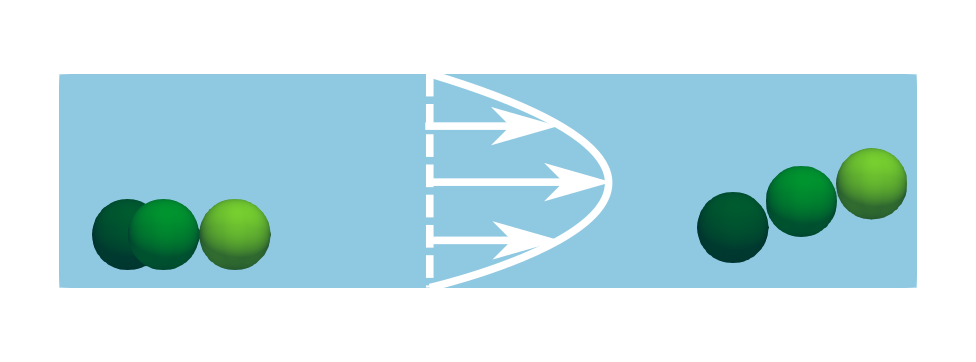
\includegraphics[width=.7\columnwidth]{../paper2/figs/3-line-side1.png}
        \vskip0.3cm
        With depletion force: forming a chain.
      } % end only
      \only<4>{
        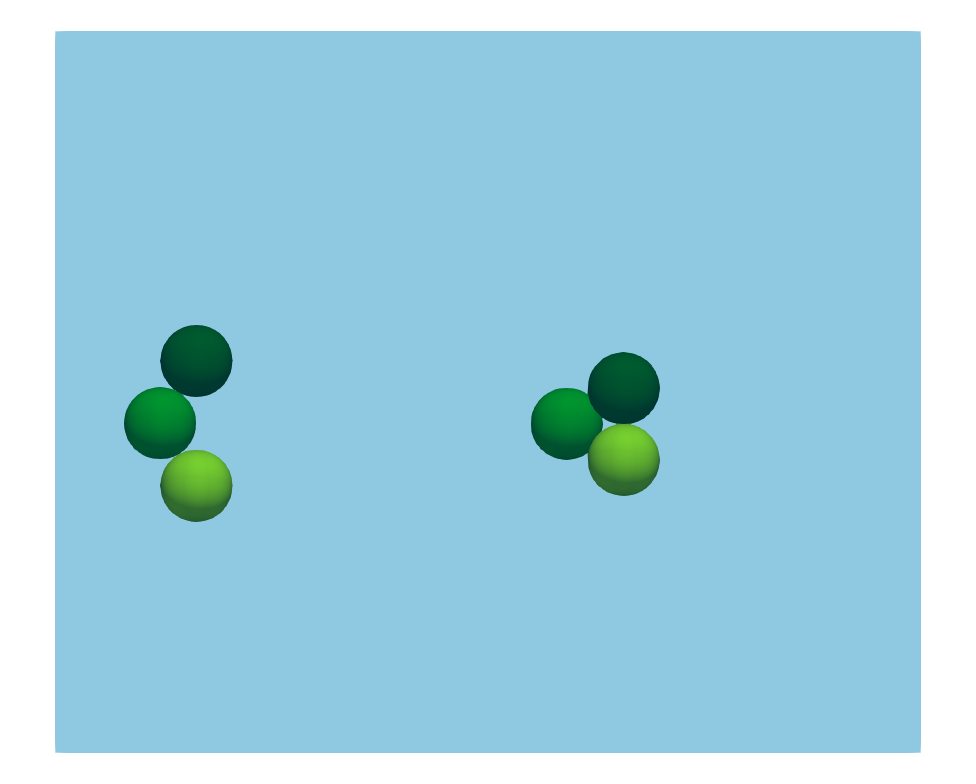
\includegraphics[width=.7\columnwidth]{../paper2/figs/3-triangle-top.png}
        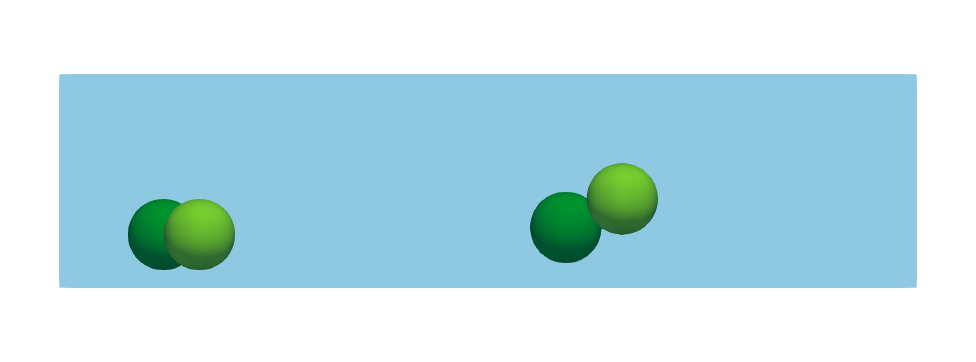
\includegraphics[width=.7\columnwidth]{../paper2/figs/3-triangle-side.png}
        \vskip0.3cm
        With depletion force: forming a triangle.
      } % end only
      \only<5>{
        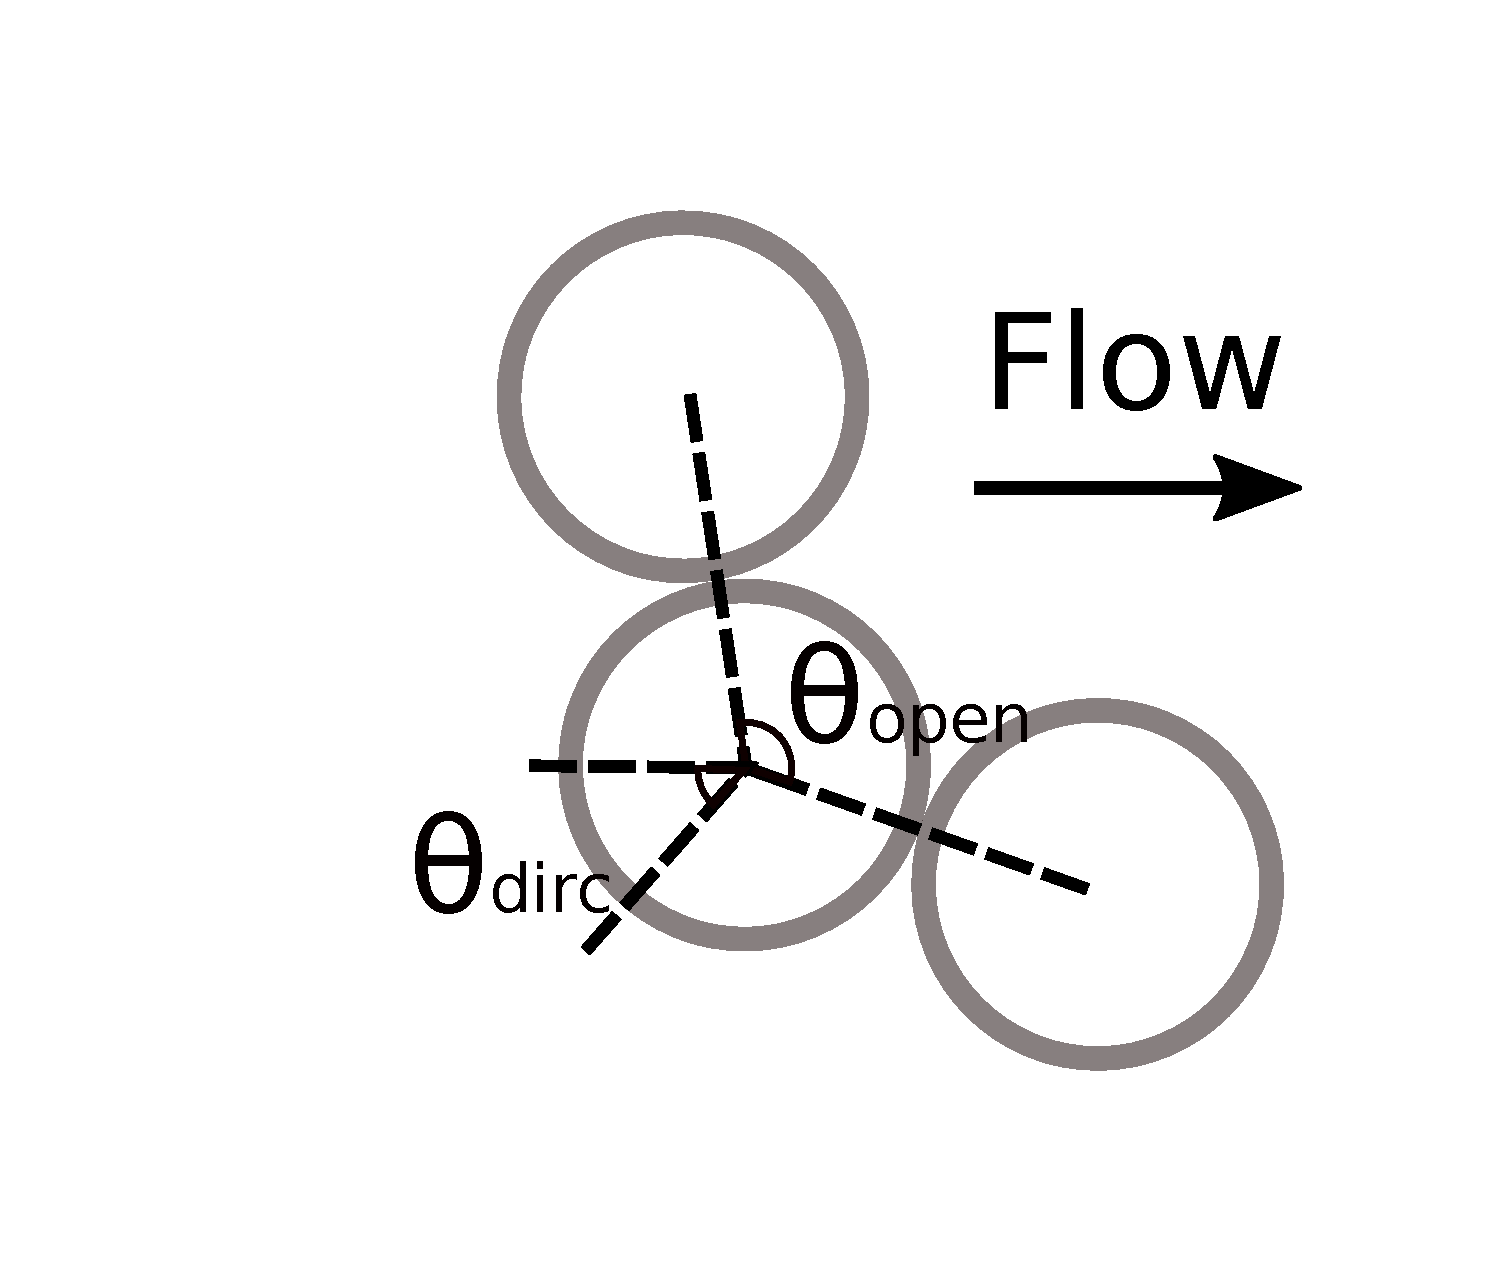
\includegraphics[width=.5\columnwidth]{../paper2/figs/angle_sketch1.pdf}
        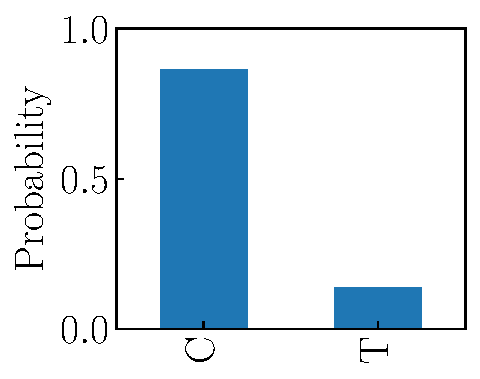
\includegraphics[width=.5\columnwidth]{../paper2/figs/result_poi_bar.pdf}
        \vskip0.3cm
        Overall, chains are more favorable than triangles.
      } % end only
      \only<6>{
        \vskip1cm
        \movie[]{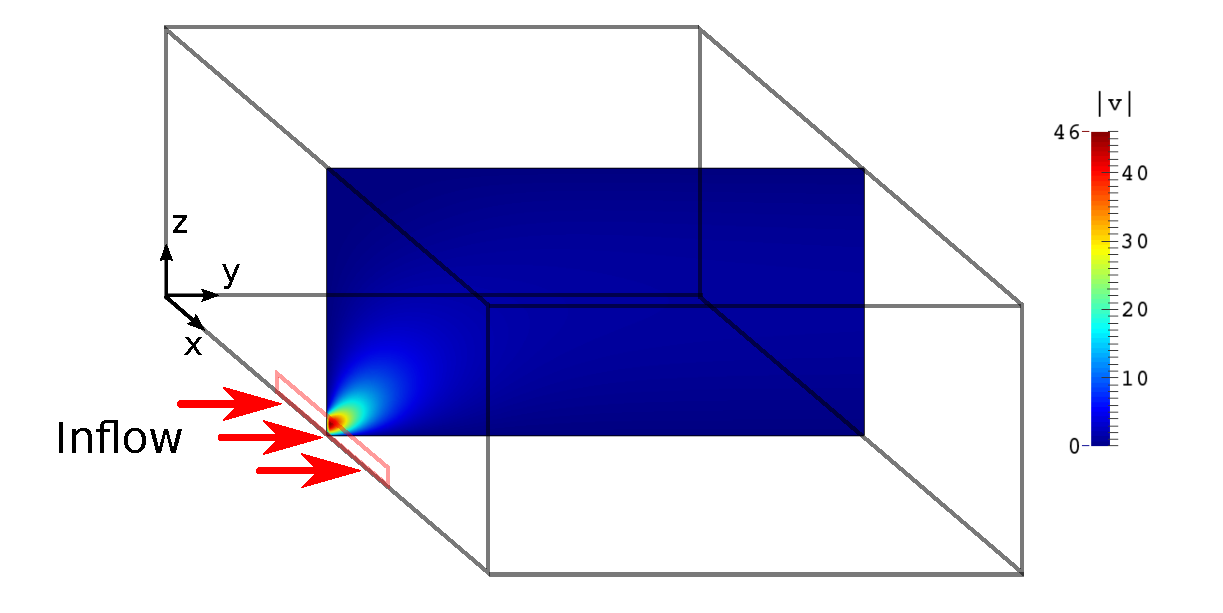
\includegraphics[width=\columnwidth]{../paper2/figs/non-uniform_inflow1.pdf}}
              {videos/movie-bird.ogv}
        \vskip0.3cm
        A very non-uniform inflow.
      } % end only
      \only<7-8>{
        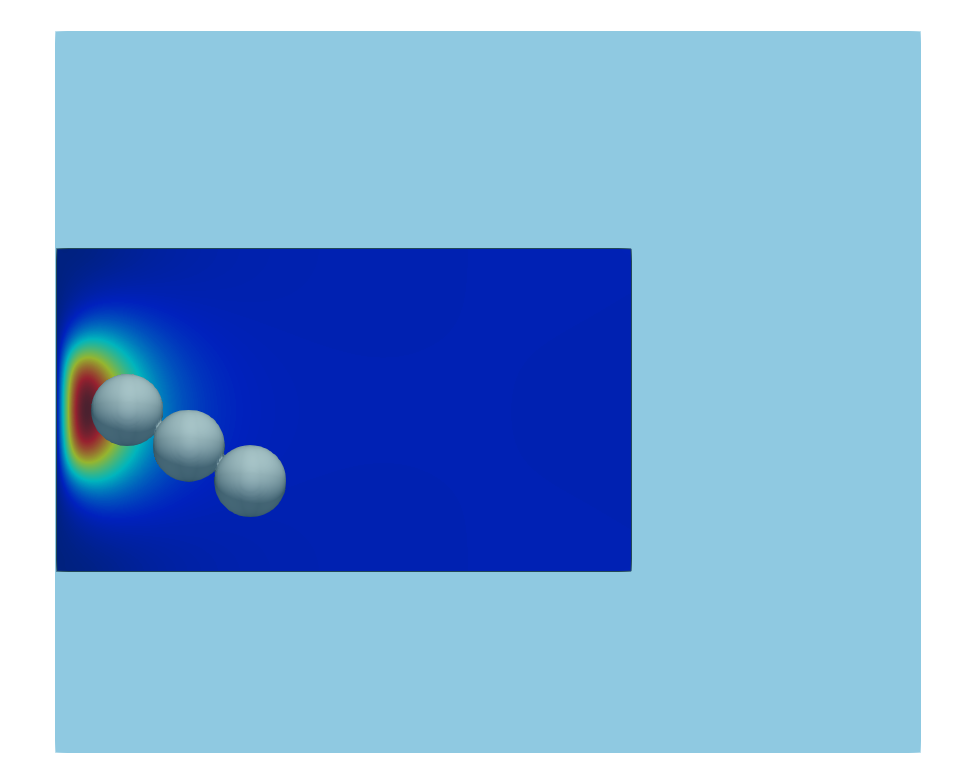
\includegraphics[width=.32\columnwidth]{../paper2/figs/bx6-top-0.png}
        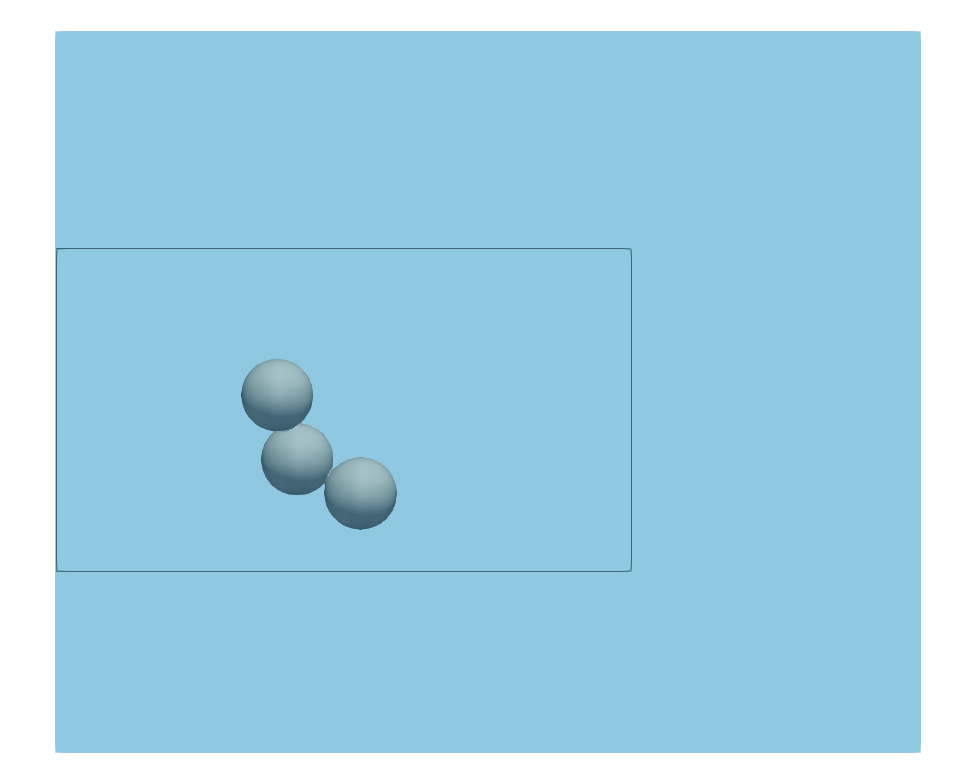
\includegraphics[width=.32\columnwidth]{../paper2/figs/bx6-top-150k-l.png}
        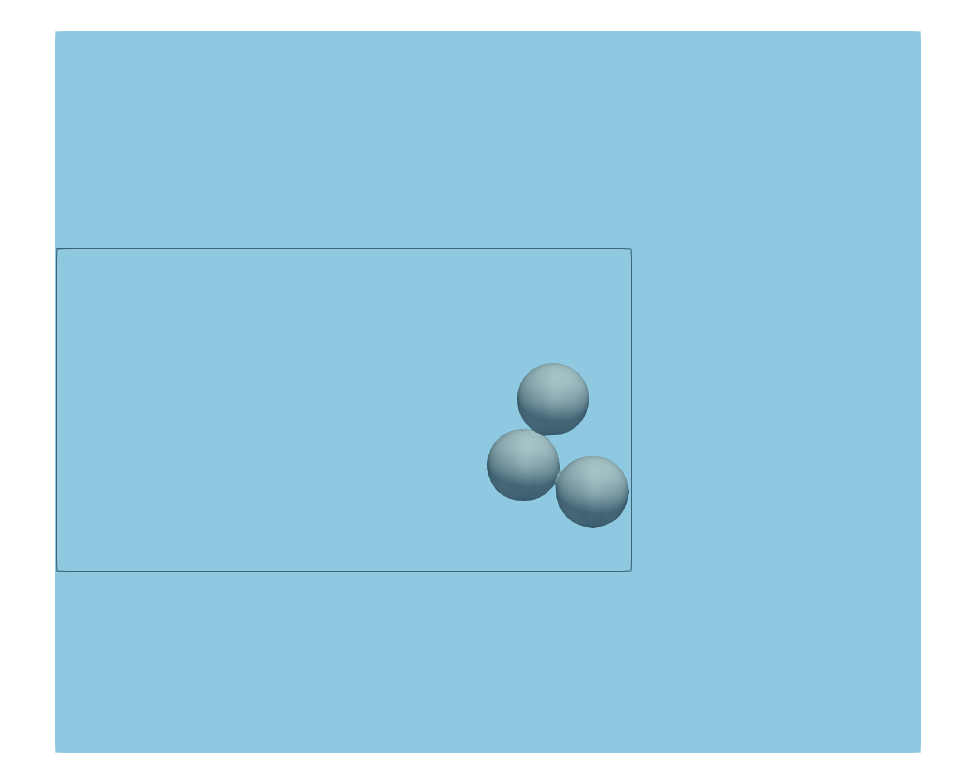
\includegraphics[width=.32\columnwidth]{../paper2/figs/bx6-top-570k.png}
        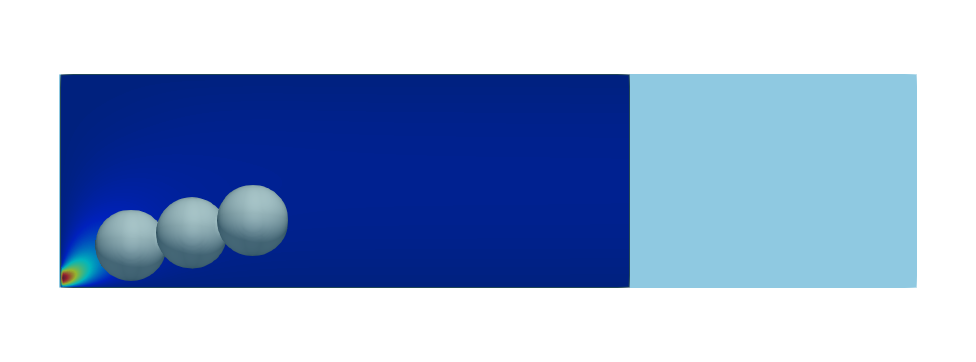
\includegraphics[width=.32\columnwidth]{../paper2/figs/bx6-side-0.png}
        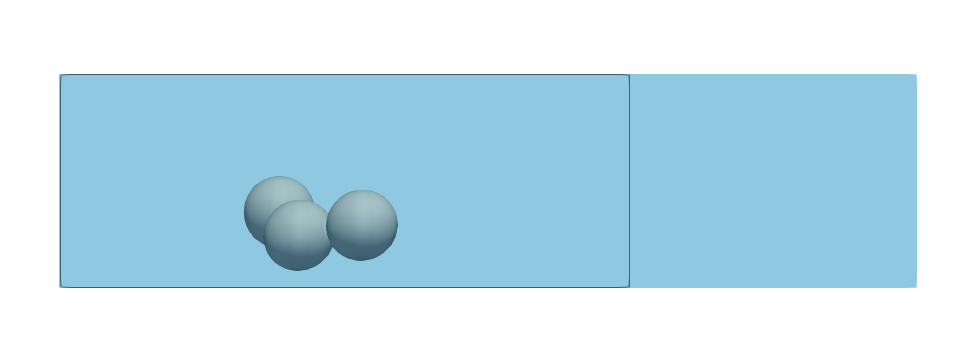
\includegraphics[width=.32\columnwidth]{../paper2/figs/bx6-side-150k-l.png}
        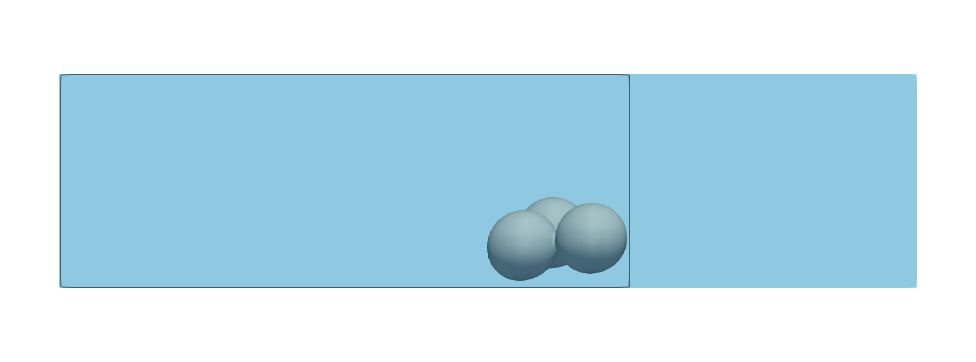
\includegraphics[width=.32\columnwidth]{../paper2/figs/bx6-side-570k.png}
        
\includegraphics[width=.75\columnwidth]{../paper2/figs/time_arrow.pdf}
        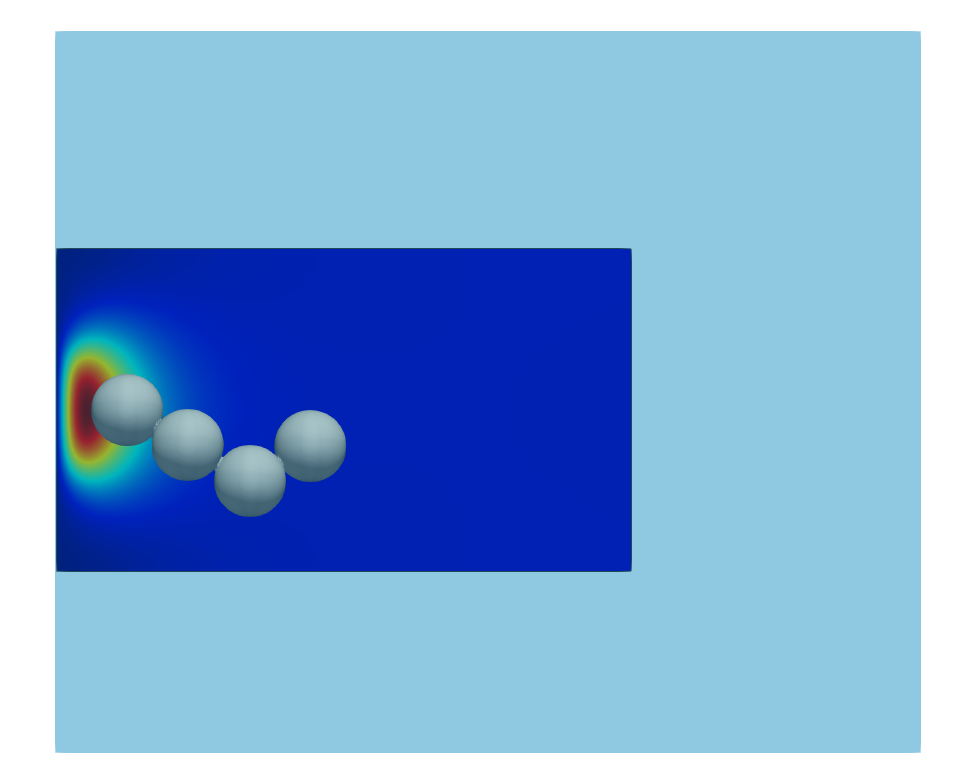
\includegraphics[width=.32\columnwidth]{../paper2/figs/bd8-top-0.png}
        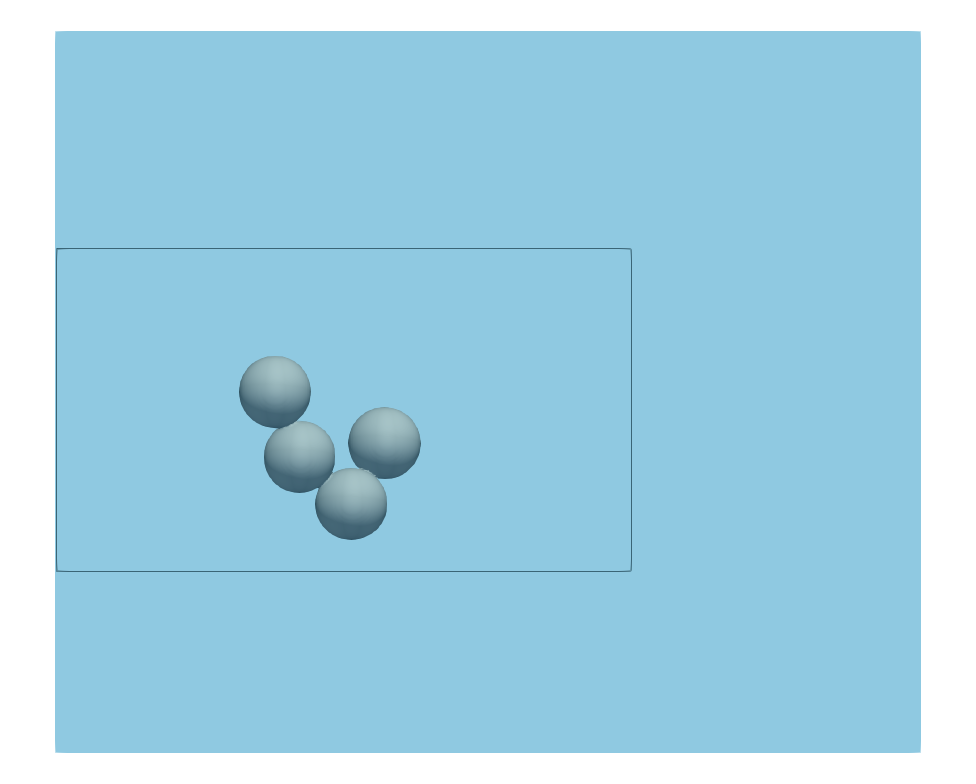
\includegraphics[width=.32\columnwidth]{../paper2/figs/bd8-top-150k.png}
        \includegraphics[width=.32\columnwidth]{../paper2/figs/bd8-top-450k.png}
        \includegraphics[width=.32\columnwidth]{../paper2/figs/bd8-side-0.png}
        \includegraphics[width=.32\columnwidth]{../paper2/figs/bd8-side-150k.png}
        \includegraphics[width=.32\columnwidth]{../paper2/figs/bd8-side-450k.png}
        \vskip0.1cm
        Assembly of 3-4 droplets.
      } % end only
      \end{figure}
    \end{column}
    
  \end{columns}
  
\end{frame}

%%
\begin{frame}[t]
  \frametitle{Flow-assisted assembly: But what about the dipolar interactions?}

  \begin{columns}[T]
    
    \begin{column}{0.45\textwidth}
      \centering
      \only<1>{
        \includegraphics[height=4cm]{imgs/espci-chip-cartoon.png}
        \includegraphics[height=2.8cm]{imgs/espci-dipolar-cartoon.png}
      } % end only
      \only<2->{
        \begin{figure}
          \includegraphics[width=\columnwidth]{../paper3/flow_vort-40k_small.pdf}
          \caption{Depth-averaged disturbance flow around a sphere travelling in the $x'$ direction.
            The particle is located in the middle of a pressure-driven channel with $H/D=1.5$.%
            \footnote<2->[frame]{Fouxon \etal Phys. Rev. E. 96, 063110 (2017).}}
        \end{figure}
      } %end only
    \end{column}

    \begin{column}{0.45\textwidth}
      
      \begin{bluecolorbox}[Obersvations \& hypotheses]
        \begin{itemize}
        \item Droplets are in quasi-two-dimensional (q2D) space.
        \item Depletion force attracts nearby drops.
        \item Hydrodynamic interactions (HI) lead to the rearrangement dynamics.
        \end{itemize}
      \end{bluecolorbox}

      \vskip.3cm
      \begin{bluecolorbox}[Equations of motion (due to HI)]
        \begin{equation} \notag
          \begin{aligned}
            & {\bm u}^\infty(x,y,z) \approx -\frac{z(H-z)}{2\mu} \nabla p(x,y), \\
            & \delta{\bm u}_{ij} = {\bm B}_{ij} {\bm F}_j, \quad {\bm U}_i = {\bm u}^\infty_i + \sum_{j \ne i} \delta{\bm u}_{ij},
          \end{aligned}
        \end{equation}
        where
        \begin{equation} \notag
          \begin{aligned}
            {\bm B}({\bm x}) \approx -\frac{\alpha H}{\mu} \bigg( \frac{{\bm I}}{\abs{\bm x}^2} -
            \frac{ 2{\bm x}{\bm x} }{ \abs{{\bm x}}^4} \bigg).
          \end{aligned}
        \end{equation}
      \end{bluecolorbox}
    \end{column}

  \end{columns}

  \only<3->{
    \begin{textblock}{80}(91,92)
      \xb{However, the prefactor is $\sim \mathcal{O}(10^{-2})$.}
    \end{textblock}
  } % end only
  
  \only<4->{
    \begin{textblock}{100}(8,87)
      \xr{\bf The picture is correct; but the number is wrong.}
    \end{textblock}
  }% end only
  
\end{frame}

%%
\hypertarget{conclusion1}{%
  \subsection{Conclusions}}

\begin{frame}[t]
  \frametitle{Conclusions}

  \vskip0.4cm
  \begin{columns}[T]
    
    \begin{column}{0.95\textwidth}
      \begin{bluecolorbox}[Droplet interactions]
        \begin{itemize}
        \item The depletion force is short-range, radial and instantaneous.
          It keeps droplets in a cluster but does not contribute to inter-cluster rearrangement. \medskip
          
        \item Confinement modifies the phase portrait of droplet trajectories.
          Combined with a strong depletion attraction, it promotes chain-like structures aligned with the flow.\medskip
          
        \item Dipolar interactions is weak in confined 3D geometries.
          An inhomogeneous inflow profile is responsible for the experimentally observed droplet clustering.\medskip
          
        \item Overall, it is difficult to calibrate all 3D effects at play.
        \end{itemize}
      \end{bluecolorbox}

      \vskip0.4cm
      \only<2->{
      \begin{bluecolorbox}[Photonic material fabrication]
        \begin{itemize}
        \item The microfluidic-based approach is theoretically possible, but tricky in practice.%
          \footnote<2->[frame]{Morozov \& Leshansky, Langmuir. 35, 11, 3987-3991 (2019).}\medskip

        \item Current trend seems to be shifted from colloidal self-assembly to making new disordered structures.%
          \footnote<2->[frame]{Ricouvier \etal PNAS. 116 (19), 9202-9207 (2019).}   
        \end{itemize}
      \end{bluecolorbox}
      } %end only
    \end{column}
      
    %\begin{column}{0.4\textwidth}
    %  \centering 
    %  \includegraphics[width=.6\columnwidth]{../imgs/photonics_cover.jpg} \vskip0.4cm
    %  \includegraphics[width=.9\columnwidth]{imgs/espci-delta.png}
    %\end{column}
  \end{columns}
  
\end{frame}

%%
\hypertarget{part2}{%
  \section{Part II: Modelling Dense Suspensions (DS)}}

%%
\hypertarget{background2}{%
  \subsection{Soft matter and rheology}}

\begin{frame}[t]
  \frametitle{Soft matter and rheology}

  
  \begin{columns}[T]
    
    \begin{column}{0.6\textwidth}
      In his Nobel lecture (1991), de Gennes described two main features of \emph{soft matter}:
      \begin{itemize}
      \item complexity (he used the analogy of biology);
      \item flexibility (he used the example of rubber).
      \end{itemize}
      \vskip0.2cm
      \only<2->{Specifically, it includes cells, polymers, surfactants, liquid crystals, colloidal grains, {\it etc.}}
      \vskip0.2cm
      \only<3->{A better understanding of these systems \xb{in} and \xr{out of} equilibrium thus has many practical relevance.}
      \vskip0.2cm
      \only<4->{In particular, a currently active area is {\bf dense suspension},
        where suspending particles occupy equal or more volume than the underlying fluid and
        interact strongly via short-range lubrication or non-hydrodynamic forces.}
      \vskip0.2cm
      \only<5->{This is intimately related to \emph{rheology}, which studies the deformation and flow of matter (in the overdamped regime).}
      \vskip0.2cm
      \only<6->{There are rich phenomena in dense suspensions, such as \xb{shear thickening} or \xb{jamming}.}
      \vskip0.2cm
      \only<7->{Questions regarding how such rheological behaviours depend on microscopic interactions or particle/manifold geometries are still unanswered today.}
    \end{column}

    \begin{column}{0.3\textwidth}      
      \vskip1cm
      \begin{figure}
        \centering
        \only<1-3>{
          \includegraphics[width=\columnwidth]{imgs/ecoli.jpg}
          \caption{E. coli, a common baterium in the gut and a model organism in biological studies.}
        } % end only
        \only<4->{
          \includegraphics[width=\columnwidth]{../paper7/figs/np2000_vol0.55.png}
          \caption{Simulation snapshot of a bidisperse suspension of 2000 spheres at 55\% volume fraction.}
        } % end only
      \end{figure}
    \end{column}
  \end{columns}

\end{frame}

%%
\hypertarget{simulation2}{%
  \subsection{Numerical modelling}}

%%
\hypertarget{hlgd}{%
  \subsubsection{HLGD}}

%%
\hypertarget{Cases}{%
  \subsection{Case studies}}

%%
\hypertarget{conclusion2}{%
  \subsection{Outlook}}

%%
\hypertarget{summary}{%
  \section{Summary}}

%%
\hypertarget{acknowledgements}{%
  \section{Acknowledgements}}










\iffalse

\begin{frame}
  \frametitle{}

  \begin{bluecolorbox}[Hypotheses for cascade directions]  
  \begin{itemize}
  \item
    In Batchelor we believe.
  \item
    Yes we still do.
  \end{itemize}  
  \end{bluecolorbox}  

\end{frame}

\fi

